\documentclass[11pt,a4paper]{article}
\usepackage[a4paper,margin=2.5cm]{geometry}
\usepackage{amsmath,amssymb,amsthm}
\usepackage{graphicx}
\usepackage{booktabs}
\usepackage{multirow}
\usepackage{longtable}
\usepackage{array}
\usepackage{hyperref}
\usepackage{xcolor}
\usepackage{listings}
\usepackage{enumitem}
\usepackage{parskip}
\usepackage{fancyhdr}
\usepackage{titlesec}

\hypersetup{
  colorlinks=true,
  linkcolor=blue!50!black,
  citecolor=blue!50!black,
  urlcolor=blue!50!black,
  pdftitle={ozGUI / ozLib: Ornstein--Zernike Solver Toolkit},
  pdfauthor={ozGUI/ozLib project}
}

\lstset{
  basicstyle=\ttfamily\small,
  breaklines=true,
  frame=single,
  columns=fullflexible,
  backgroundcolor=\color{gray!8},
  keywordstyle=\color{blue!60!black},
  commentstyle=\color{green!40!black},
  stringstyle=\color{red!60!black},
  language=Python,
  showstringspaces=false
}

\pagestyle{fancy}
\fancyhf{}
\fancyhead[L]{ozGUI / ozLib Documentation}
\fancyhead[R]{\thepage}
\renewcommand{\headrulewidth}{0.4pt}

\newtheorem{remark}{Remark}

\newcommand{\code}[1]{\texttt{#1}}

\title{\bfseries ozGUI / ozLib\\[2mm]
Ornstein--Zernike Solver Toolkit\\[1mm]
\large including the multicomponent and polydisperse extension}
\author{ozGUI/ozLib project}
\date{\today}

\begin{document}
\maketitle
\tableofcontents
\clearpage
\part{The one-component toolkit}


\thispagestyle{empty}




\clearpage

\section{Overview}

\code{ozGUI}/\code{ozLib} solves the Ornstein--Zernike (OZ) integral equation for a
single-component, isotropic fluid of spherically symmetric particles, given
\begin{itemize}[nosep]
  \item a pair interaction potential $U(r)$ (Section~\ref{sec:potentials}),
  \item a closure relation connecting the direct correlation function $c(r)$ to
        the total correlation function $h(r)=g(r)-1$ (Section~\ref{sec:closures}),
  \item a volume fraction $\varphi$, and
  \item a numerical solver algorithm that finds the self-consistent fixed point
        of the resulting nonlinear system (Section~\ref{sec:solvers}).
\end{itemize}
The output is the pair correlation function $g(r)$, the direct correlation
function $c(r)$, the static structure factor $S(q)$, and several auxiliary
quantities (the cavity function $y(r)$, the bridge function $B(r)$, the
indirect correlation function $\Gamma(r)=h(r)-c(r)$, and the reduced potential
$U(r)/k_BT$).

Two front ends share the exact same computational core (\code{ozLib.py}), so
results obtained through either are identical by construction:
\begin{itemize}[nosep]
  \item \textbf{\code{oZgui.py}} --- an interactive Tkinter application with
        potential/closure/solver dropdowns, a 9-tab plot panel, run history,
        and Save/Load/ASCII/CSV/Excel/PNG export (Section~\ref{sec:gui}).
  \item \textbf{\code{ozLib.py}} --- a plain Python function,
        \code{ozLib.solve(...)}, usable directly in scripts without any GUI
        dependency (Section~\ref{sec:ozlib}).
\end{itemize}

\section{The Ornstein--Zernike Equation and its Discretisation}
\label{sec:theory}

\subsection{The OZ equation}

For an isotropic, single-component fluid the Ornstein--Zernike equation reads,
in real space,
\begin{equation}
  h(r) = c(r) + \rho \int c(|\mathbf{r}-\mathbf{r}'|)\, h(r')\, d\mathbf{r}',
\end{equation}
where $\rho$ is the number density and the convolution is over all space.
Introducing the indirect correlation function $\Gamma(r) \equiv h(r)-c(r)$, and
Fourier--Bessel (Hankel) transforming (exploiting isotropy to reduce the 3D
Fourier transform to a 1D sine transform), the OZ equation becomes purely
algebraic in reciprocal space,
\begin{equation}
  \hat\Gamma(q) = \frac{\hat c(q)}{1-\rho\,\hat c(q)} - \hat c(q),
  \label{eq:oz-fourier}
\end{equation}
where $\hat f(q)$ denotes the (3D, spherically-symmetric) Fourier transform of
$f(r)$. The OZ equation alone relates two unknowns, $c(r)$ and $h(r)$ (or
equivalently $\Gamma(r)$); a second, independent relation --- the
\emph{closure} --- is required to close the system. Every closure implemented
here has the general form
\begin{equation}
  c(r) = f\big(\Gamma(r), U(r)\big)
\end{equation}
for some function $f$ specific to the closure (Section~\ref{sec:closures}). The
full problem is therefore a fixed-point problem in $\Gamma(r)$ (or, in an
equivalent formulation used by some solvers here, in $c(r)$ and $h(r)$
jointly): starting from a trial $\Gamma(r)$, the closure gives $c(r)$, the OZ
equation (Eq.~\ref{eq:oz-fourier}) gives a new $\Gamma(r)$, and a solver
algorithm (Section~\ref{sec:solvers}) drives this map to self-consistency.

\subsection{Discrete grid: real space}

The real-space grid is a plain equal-spaced grid of $N=\code{numberOfRadialSamplingPoints}$
points,
\begin{equation}
  r_i = i\,\Delta r, \qquad i=1,2,\dots,N,
\end{equation}
starting at $\Delta r$ rather than $0$ (division by $r$ appears in the Hankel
transform below, so $r=0$ is avoided by construction rather than special-cased).
The hard-core diameter $\sigma$ is placed at grid index
$\code{hardSphereDiameterInPoints}$ (called $n_\sigma$ below), i.e.
\begin{equation}
  \sigma = n_\sigma\,\Delta r, \qquad
  \text{total range } r_{\max} = (N-1)\Delta r = \frac{N-1}{n_\sigma}\,\sigma.
\end{equation}
Both $N$ and $n_\sigma$ are configurable (constructor keyword arguments
\code{numberOfRadialSamplingPoints}, \code{hardSphereDiameterInPoints} on every
solver class, and identically-named arguments on \code{ozLib.solve()}); the
historical defaults are $N=4096$, $n_\sigma=100$, giving $r_{\max}\approx
41\,\sigma$ and $\Delta r = 0.01\,\sigma$. Increasing $N$ at fixed $n_\sigma$
extends the range without losing near-contact resolution --- important for
slowly-decaying, long-range potentials (e.g.\ small-$\kappa$ Yukawa/DLVO tails),
where a too-short grid truncates the potential before it has actually decayed
to zero, distorting $S(q)$ at low $q$ (this was verified directly: a 4$\times$
extension of the default grid reduced a Yukawa potential's residual value at
the grid edge from $\mathcal{O}(10^{-4})\,k_BT$ to $\mathcal{O}(10^{-10})\,k_BT$,
and changed $S(q\!\to\!0)$ by about 33\%).

\subsection{Discrete Hankel transform}

For an isotropic function $f(r)$ the 3D Fourier transform reduces to
\begin{equation}
  \hat f(q) = \frac{4\pi}{q}\int_0^\infty r\,f(r)\,\sin(qr)\,dr,
\end{equation}
which is implemented here as a type-I discrete sine transform (DST) of
$r_i f(r_i)$, following the same construction documented in SASfit's own
theory notes (equations 5.18/5.19 there):
\begin{equation}
  \hat f(q_k) = \frac{2\pi \Delta r^2}{\Delta q}\cdot
                \frac{\mathrm{DST\text{-}I}\big[r_i f(r_i)\big]_k}{k},
  \qquad
  \Delta q = \frac{\pi}{(N+1)\Delta r},
  \qquad q_k = k\,\Delta q.
\end{equation}
The inverse transform is the same operation up to a normalisation factor
($\Delta q^3/[(2\pi)^3\Delta r^3]$), since the Hankel transform pair is (up to
constants) self-inverse. Both directions are implemented once, in
\code{OZfixpointOperator.hankelTransform()}/\code{inverseHankelTransform()},
and shared by every closure and every solver.

\subsection{Grand-canonical thermodynamic quantities}

For the hard-sphere/Percus--Yevick case, the exact grand-canonical
compressibility-route structure factor at $q=0$ is available in closed form
(used as an internal consistency check, e.g.\ in RMSA's own bisection, see
Section~\ref{sec:rmsa-closure}):
\begin{equation}
  S(q\!=\!0) = \frac{(1-\varphi)^4}{(1+2\varphi)^2}.
\end{equation}

\section{Interaction Potentials}
\label{sec:potentials}

Every potential is specified through its Boltzmann factor
$\exp[-U(r)/k_BT]$ (stored as \code{boltzmannOfP2Ppotential}), evaluated on the
grid described above; all energies are in $k_BT$ units and all lengths in units
where the hard-core diameter is $\sigma=n_\sigma\Delta r$. Potentials that
support the repulsive/attractive potential split needed by
switching-function closures (Rogers--Young, HMSA, and the Gstar-based bridge
closures of Section~\ref{sec:closures}) additionally populate the arrays
\code{repulsivePartOfP2Ppotential} and \code{attractivePartOfP2Ppotential}.
All 18
potentials below are available via \code{setPotentialByName(name, *args)} or
directly as \code{set<Name>Potential(...)} -- in 17 subsections, not 18,
since Section~\ref{sec:starpolymer} covers both of the star polymer
potential's two distinct setters (\code{setStarPolymerHighFPotential()},
\code{setStarPolymerLowFPotential()}) together, one formula each.

\emph{Note on counting, and on a genuine fix this made:} the GUI's own
potential dropdown (Table~\ref{tab:potential-naming},
Section~\ref{sec:tcl-comparison}) lists 18 named entries. An earlier version
of this port had only 17 setters -- \code{setStarPotential()} implemented
only the star polymer potential's $f\ge10$ formula, silently applied
regardless of functionality, with no $f\le10$ counterpart at all,
unlike the original Tcl GUI's two separate \code{StarPolymer (f>10)}/
\code{StarPolymer (f<10)} dropdown entries. Checking
\code{sasfit\_oz\_potential\_star\_Likos.c} directly (rather than assuming
the single existing formula covered every $f$) found this is a genuinely
different second formula (\code{U\_Star2}, Section~\ref{sec:starpolymer}),
not just the same one evaluated at a smaller argument -- now added as
\code{setStarPolymerLowFPotential()}, matching the Tcl GUI's count exactly.
\code{Depl-Sph-Sph}/\code{Depl-Sph-Discs}/\code{Depl-Sph-Rods} similarly
appear as three separate GUI choices against one Depletion subsection here
-- checked the same way the star polymer case was: confirmed to be a
similarly-missing split (see Section~\ref{sec:depletion}'s own
\textbf{Known gap} note), not a single shared formula with different
constant substitutions, though unlike star polymer this one was found but
not fixed in this pass.

\subsection{Hard Sphere}
\begin{equation}
  \exp[-U(r)/k_BT] = \begin{cases} 0 & r<\sigma \\ 1 & r\ge\sigma. \end{cases}
\end{equation}

\subsection{Lennard-Jones}
\begin{equation}
  U(r)/k_BT = 4\varepsilon\left[\left(\frac{\sigma}{r}\right)^{12}-\left(\frac{\sigma}{r}\right)^{6}\right],
\end{equation}
with $\varepsilon$ in $k_BT$ units. The potential is split at its minimum
($r_{\min}=2^{1/6}\sigma$) into a repulsive part ($r<r_{\min}$) and an
attractive part ($r\ge r_{\min}$), for use by switching-function closures.

\subsection{Yukawa (screened Coulomb), with optional hard core}
\begin{equation}
  U(r)/k_BT = K\,\frac{\sigma}{r}\,e^{-r/\lambda},
\end{equation}
where $\lambda$ is the screening length (in units of $\sigma$) and $K$ the
contact interaction strength; a hard core can optionally be added
(\code{doAddHardSphere}), in which case the exponential and $1/r$ factors are
shifted independently as in SASfit's own construction, and the potential is
set to $\infty$ (Boltzmann factor 0) for $r<\sigma$.

\subsection{Star polymer potential (Likos \& Harreis) \cite{likos2002}}
\label{sec:starpolymer}
Two genuinely different formulas, one for each of two functionality
regimes, matching \code{U\_Star1} and \code{U\_Star2} in
\code{sasfit\_oz\_potential\_star\_Likos.c} respectively. This port calls
them \code{setStarPolymerHigh\-FPotential()} and
\code{setStarPolymerLow\-FPotential()}; an earlier version only had the
first of these, silently applying it regardless of $f$.


\textbf{High functionality, $f\ge10$} (exponential decay outside the core):
\begin{equation}
  U(r)/k_BT =
  \begin{cases}
    \dfrac{5}{18}f^{3/2}\left[-\ln\!\dfrac{r}{\sigma}+\dfrac{1}{1+\sqrt{f}/2}\right] & r\le\sigma\\[2ex]
    \dfrac{5}{18}f^{3/2}\,\dfrac{1}{1+\sqrt{f}/2}\,\dfrac{\sigma}{r}\,
      \exp\!\left[-\dfrac{\sqrt{f}(r-\sigma)}{2\sigma}\right] & r>\sigma.
  \end{cases}
\end{equation}

\textbf{Low functionality, $f\le10$} (Gaussian decay outside the core, with
its own $\tau(f)$ interpolation):
\begin{equation}
  \tau(f) = \tau_2 + \frac{\tau_5-\tau_2}{3}f, \qquad
  \tau_2 = \frac{1.03}{\sigma}, \quad \tau_5 = \frac{1.12}{\sigma},
\end{equation}
\begin{equation}
  U(r)/k_BT =
  \begin{cases}
    \dfrac{5}{18}f^{3/2}\left[-\ln\!\dfrac{r}{\sigma}+\dfrac{1}{2(\tau\sigma)^2}\right] & r\le\sigma\\[2ex]
    \dfrac{5}{18}f^{3/2}\,\dfrac{1}{2(\tau\sigma)^2}\,
      \exp\!\left[-\tau^2(r^2-\sigma^2)\right] & r>\sigma.
  \end{cases}
\end{equation}
Here $f=$ \code{NumberOfArms} is the number of arms of the star polymer
(the same argument name on both setters). The two branches do \emph{not}
meet smoothly at $f=10$ -- checked directly: $\sim$28\% relative
difference in $U(r=\sigma^+)$, about 30$\times$ apart by $r=2\sigma$.
This is a genuine property of the original paper's own two-regime fit
(each branch is only claimed accurate within its own stated range), not
a bug in either formula or this port; $f=10$ is where Likos \& Harreis
recommend switching approximations, not a point the two forms were
designed to agree at exactly. A caller choosing between the two should
therefore pick whichever branch matches their actual $f$, not assume
either extrapolates sensibly across the boundary.

\subsection{Depletion potential (Oversteegen \& Lekkerkerker) \cite{oversteegen2004}}
\label{sec:depletion}
Two-sphere overlap-volume depletion potential between big spheres (diameter
$\sigma_1=\sigma$, the species this OZ solve is for) induced by small
depletant spheres (diameter $\sigma_2=$ \code{sigmaRatio}$\cdot\sigma_1$, number
density $\rho_2$ set via the depletant volume fraction \code{phi2}):
\begin{equation}
  U(r)/k_BT = -\rho_2\,\frac{\pi\sigma_1^3(1+r_t)^3}{6}
  \left[1-\frac{3r}{2(1+r_t)\sigma_1}+\frac{r^3}{2(1+r_t)^3\sigma_1^3}\right],
  \qquad \sigma_1\le r<\sigma_1+\sigma_2,
\end{equation}
with $r_t=\sigma_2/\sigma_1$, and $U=0$ for $r\ge\sigma_1+\sigma_2$; hard core
for $r<\sigma_1$.

\textbf{Known gap, found while cross-checking the star polymer split of
Section~\ref{sec:starpolymer} prompted a closer look at this file too:}
\code{sasfit\_oz\_potential\_depletion.c} actually contains \emph{four}
distinct formulas, not one -- the generic \code{U\_Depletion} above, plus
\code{U\_DepletionOfSpheresBySpheres}, \code{U\_DepletionOfSpheresByDiscs},
and \code{U\_DepletionOfSpheresByRods}, matching the Tcl GUI's own three
named dropdown entries (\code{Depl-Sph-Sph}/\code{Depl-Sph-Discs}/
\code{Depl-Sph-Rods}, Table~\ref{tab:potential-naming},
Section~\ref{sec:tcl-comparison}) -- each geometrically distinct (sphere
depleted by spheres/discs/rods respectively, the disc and rod cases
involving genuinely different overlap-volume geometry, e.g.\ an
$\arcsin$ term for discs) and parametrised differently from
\code{U\_Depletion} (\code{sigma\_large}, \code{sigma\_small}/\code{D}/\code{L},
and a number density \code{nb} directly, rather than
\code{sigma1}/\code{sigma2}/a volume fraction \code{PHI2}). This Python port
currently only has the generic \code{U\_Depletion} form -- unlike the star
polymer fix of Section~\ref{sec:starpolymer}, this was found but
deliberately \emph{not} fixed in this pass (out of the scope of what was
asked, and a larger, riskier addition: three new geometries to verify,
not one), and is recorded here so it isn't silently lost.

\subsection{DLVO (electrostatic double-layer + van der Waals)}
\label{sec:dlvo}
\begin{equation}
  U(r)/k_BT = U_{\mathrm{el}}(r) + U_{\mathrm{vdW}}(r), \qquad r>\sigma,
\end{equation}
\begin{equation}
  U_{\mathrm{el}}(r) = \frac{L_B Z^2}{(1+\kappa a)^2}\,\frac{e^{-\kappa(r-\sigma)}}{r},
  \qquad
  U_{\mathrm{vdW}}(r) = -\frac{A}{6}\left[\frac{2a^2}{r^2-4a^2}+2\left(\frac{a}{r}\right)^2
    +\ln\!\left(1-4\Big(\frac{a}{r}\Big)^2\right)\right],
\end{equation}
where $a=\sigma/2$, $\kappa$ the inverse Debye screening length, $Z$ the
macro-ion charge, $L_B$ the Bjerrum length, and $A$ the effective Hamaker
constant. $U_{\mathrm{vdW}}$'s genuine divergence at $r=\sigma$ is excluded from
the computation itself (not merely masked afterward), since the grid places a
real point at exactly $r=\sigma$.

\subsection{DLVO + hydration repulsion}
As Section~\ref{sec:dlvo}, plus a short-range exponential hydration term,
\begin{equation}
  U(r)/k_BT = U_{\mathrm{DLVO}}(r) - 2\,G_{HY}\,e^{-(r-\sigma)/D_H}, \qquad r>\sigma,
\end{equation}
with hydration strength $G_{HY}$ and decay length $D_H$.

\subsection{Fermi distribution model (Likos)}
\begin{equation}
  U(r)/k_BT = \varepsilon\,\frac{1+e^{-\sigma/\xi}}{1+e^{(r-\sigma)/\xi}}.
\end{equation}
The limit $\xi\to0$ reduces to the penetrable sphere model (below), and is
handled as a special case when $\xi=0$ is passed exactly.

\subsection{Generalized Gaussian core model (GGCM-$n$)}
\begin{equation}
  U(r)/k_BT = \varepsilon\,\exp\!\left[-\alpha\left(\frac{r}{\sigma}\right)^{n}\right].
\end{equation}

\subsection{Hard sphere + 3 additive Yukawa tails}
\begin{equation}
  U(r)/k_BT = -\frac{\sigma}{r}\sum_{i=1}^{3} K_i\,\exp\!\left[-\frac{r-\sigma}{\sigma\,\lambda_i}\right], \qquad r\ge\sigma,
\end{equation}
with hard core for $r<\sigma$; each $(K_i,\lambda_i)$ pair may be set to zero to
recover fewer effective Yukawa terms.

\subsection{Ionic microgel (Likos et al.)}
A multi-term analytical potential for a charged microgel sphere of charge $Z$,
dielectric constant $ED$, and inverse screening length $\kappa_\Pi/\sigma$
inside the gel, following Likos et al.\ (2011); the full piecewise expression
(different polynomial/hyperbolic forms inside vs.\ outside the gel radius) is
implemented exactly as in \code{sasfit\_oz\_potential\_ionic\_microgel.c} and is
reproduced verbatim in the source rather than restated here, since it spans
several auxiliary terms without a single compact closed form.

\subsection{Piecewise-constant hard-sphere shoulder/well (3 segments)}
\begin{equation}
  U(r)/k_BT =
  \begin{cases}
    \varepsilon_1 & \sigma\le r<\sigma+\delta_1\\
    \varepsilon_2 & \sigma+\delta_1\le r<\sigma+\delta_1+\delta_2\\
    \varepsilon_3 & \sigma+\delta_1+\delta_2\le r<\sigma+\delta_1+\delta_2+\delta_3\\
    0 & \text{otherwise (outside all three steps)},
  \end{cases}
\end{equation}
hard core for $r<\sigma$; each $\varepsilon_j$ may be positive (shoulder) or
negative (well). This is the general $n=3$ piecewise-constant family used as
an independent cross-check for the RFA analytical solver
(Section~\ref{sec:rfa}).

\subsection{Penetrable sphere model (Likos, Watzlawek, L\"owen) \cite{likos1998}}
\begin{equation}
  U(r)/k_BT = \begin{cases}\varepsilon & r\le\sigma\\ 0 & r>\sigma.\end{cases}
\end{equation}

\subsection{Soft sphere (inverse power law)}
\begin{equation}
  U(r)/k_BT = \varepsilon\left(\frac{\sigma}{r}\right)^{n}.
\end{equation}

\subsection{Parabolic (Hertzian) sphere}
\begin{equation}
  U(r)/k_BT = \begin{cases}\varepsilon\left(1-\dfrac{r}{\sigma}\right)^{5/2} & r\le\sigma\\ 0 & r>\sigma.\end{cases}
\end{equation}

\subsection{Square well}
\label{sec:squarewell-potential}
\begin{equation}
  U(r)/k_BT = \begin{cases} \infty & r<\sigma\\ \varepsilon & \sigma\le r\le\sigma+\delta \\ 0 & r>\sigma+\delta,\end{cases}
\end{equation}
with well width $\delta$ (well outer range $\lambda=1+\delta/\sigma$ in the
notation of Section~\ref{sec:sharma-sharma}); $\varepsilon<0$ for an attractive
well, $\varepsilon>0$ for a repulsive shoulder.

\subsection{Sticky hard sphere (Baxter's adhesive limit)}
\label{sec:stickyhs-potential}
\begin{equation}
  U(r)/k_BT = \begin{cases} \infty & r<\sigma\\ \ln\!\left(\dfrac{12\,\tau\,\delta}{\sigma+\delta}\right) & \sigma\le r\le\sigma+\delta\\ 0 & r>\sigma+\delta,\end{cases}
\end{equation}
using Baxter's stickiness parameter $\tau$ (small $\tau$ = sticky, large $\tau$
= hard-sphere limit) and a finite well width $\delta$ --- the same $\tau$
convention as SASfit's own \code{robertus\_shs} plugin, giving a natural point
of comparison between this (monodisperse, OZ-based) solve and that
(polydisperse, PY-only, multicomponent) one.

\clearpage
\section{Closure Relations}
\label{sec:closures}

Every closure below expresses $c(r)$ as a function of $\Gamma(r)$ (and, for the
switching-function and Gstar-based closures, the potential's own
repulsive/attractive split) and is dispatched through
\code{OZfixpointOperator.update\_c()}. Formulas were cross-checked directly
against SASfit's own \code{sasfit\_oz\_solver.c} \code{case} statements (not
re-derived from a textbook), using that file's own notation:
$\mathrm{EN}(r)=\exp[-U(r)/k_BT]$, $G(r)=\Gamma(r)$. Where a closure needs an
extra scalar parameter (shared storage slot \code{self.alpha}, matching the
C code's own \code{sBPGG}/\code{aCJVM}/\code{fBB} \code{\#define}s onto the
same underlying variable), this is noted explicitly. \textbf{20 closures are
offered} -- 19 general-purpose ones plus ZSEP (Section~\ref{sec:zsep}, hard
spheres only, self-fitting its own three free parameters rather than taking
any of them from the caller); a 21st (Euler--Rahman) exists in the source
but is deliberately excluded from both the GUI and \code{ozLib.solve()}'s
validated closure list -- see Section~\ref{sec:eurah} for why.

\subsection{Percus--Yevick (PY)}
\begin{equation}
  c(r) = \mathrm{EN}(r)\big[1+\Gamma(r)\big] - \Gamma(r) - 1.
\end{equation}
Equivalent to the standard PY form $c(r)=\big(e^{-U/k_BT}-1\big)y(r)$ with
cavity function $y(r)=g(r)e^{U/k_BT}$.

\subsection{Hypernetted Chain (HNC)}
\begin{equation}
  c(r) = \mathrm{EN}(r)\,e^{\Gamma(r)} - \Gamma(r) - 1.
\end{equation}

\subsection{Reference HNC (RHNC)}
\label{sec:rhnc}
Needs a reference-system sub-solve: a bare hard sphere of the same $\sigma$ is
first solved with the Martynov--Sarkisov closure (Section~\ref{sec:ms}),
giving reference cavity/indirect-correlation functions $g_0(r)$, $\Gamma_0(r)$.
Writing the actual potential's perturbation as
$\Delta U(r)/k_BT = -\ln\mathrm{EN}(r)$ (zero inside the reference hard core),
the closure is
\begin{equation}
  c(r) = g_0(r)\,\exp\!\big[\big(\Gamma(r)-\Gamma_0(r)\big) - \Delta U(r)/k_BT\big] - \Gamma(r) - 1.
\end{equation}
This reduces to the same hard-core exclusion every other hard-sphere closure
uses automatically, since $g_0(r)\equiv0$ inside the reference hard core.
Orchestrated by \code{OZsolver.solveRHNC()}.

\subsection{Modified HNC (MHNC)}
HNC plus a fixed, purely analytical Percus--Yevick hard-sphere bridge function
$B_{\mathrm{PY}}(r;\eta)$ (no reference-system sub-solve needed, unlike RHNC,
since $B_{\mathrm{PY}}$ has a closed form):
\begin{equation}
  c(r) = \mathrm{EN}(r)\,\exp\!\big[\Gamma(r) + B_{\mathrm{PY}}(r;\eta)\big] - \Gamma(r) - 1,
\end{equation}
with the packing-fraction-like parameter $\eta$ supplied by the user
(\code{doMHNCclosure(eta)}).

\subsection{Mean Spherical Approximation (MSA)}
\begin{equation}
  c(r) = \begin{cases} -\big[\Gamma(r)+1\big] & r<\sigma \quad\text{(forces }g(r){=}0)\\
    -U(r)/k_BT = \ln\mathrm{EN}(r) & r\ge\sigma. \end{cases}
\end{equation}

\subsection{Rescaled MSA (RMSA)}
\label{sec:rmsa-closure}
Identical formula to MSA, but the inside/outside switch is driven by an
\emph{apparent} hard-core gate $g_{4g}(r)\in\{0,1\}$ rather than the bare
potential's own hard core:
\begin{equation}
  c(r) = \begin{cases} -\big[\Gamma(r)+1\big] & g_{4g}(r)=0\\ \ln\mathrm{EN}(r) & g_{4g}(r)=1. \end{cases}
\end{equation}
\code{OZsolver.solveRMSA()} first solves plain MSA; if the resulting
$g(\sigma^+)<0$ (an unphysical result plain MSA can give for strongly-coupled
systems), it re-solves with the apparent hard core bisected outward, grid
point by grid point, until $g$ at the new apparent contact point is
non-negative. This is the same Hayter--Penfold-style rescaling idea underlying
Section~\ref{sec:hayter-penfold}'s semi-analytical RMSA solver, applied here
inside the general numerical OZ solve instead of via the closed-form
Hayter--Penfold machinery.

\subsection{Modified MSA (mMSA)}
As MSA, but using the Mayer function outside the core instead of the bare
potential:
\begin{equation}
  c(r) = \begin{cases} -\big[\Gamma(r)+1\big] & r<\sigma\\ \mathrm{EN}(r)-1 & r\ge\sigma. \end{cases}
\end{equation}

\subsection{``Symmetric'' MSA (SMSA)}
Using $\Gamma^*(r)=\Gamma(r)-U_{\mathrm{attr}}(r)/k_BT$ (the attractive-part-subtracted
indirect correlation function, shared with several closures below):
\begin{equation}
  c(r) = \exp\!\big[U_{\mathrm{attr}}(r)/k_BT\big]\big[\Gamma^*(r)+1\big] - \Gamma(r) - 1.
\end{equation}

\subsection{Rogers--Young (RY) \cite{rogersyoung1984}}
Interpolates between PY ($\alpha\to\infty$) and HNC ($\alpha\to0$) via a
switching function $f(r)=1-e^{-\alpha r}$:
\begin{equation}
  c(r) = \mathrm{EN}(r)\left[1+\frac{e^{f(r)\Gamma(r)}-1}{f(r)}\right] - \Gamma(r) - 1,
\end{equation}
with $\alpha$ supplied by the user (\code{doRYclosure(alpha)}).

\subsection{HMSA (Zerah--Hansen) \cite{zerahhansen1986}}
Same switching-function structure as RY, but using $\Gamma^*(r)$ in the
switching term and the full Boltzmann factor split into repulsive/attractive
parts:
\begin{equation}
  c(r) = \exp\!\big[-U_{\mathrm{rep}}(r)/k_BT\big]\left[1+\frac{e^{f(r)\Gamma^*(r)}-1}{f(r)}\right] - \Gamma(r) - 1,
\end{equation}
with $\alpha$ (in $f(r)=1-e^{-\alpha r}$) supplied by the user
(\code{doHMSAclosure(alpha)}).

\subsection{Verlet \cite{verlet1980,verlet1981}}
Empirical bridge function, no reference system or extra parameter:
\begin{equation}
  B(r) = \frac{-\Gamma(r)^2}{2\big[1+0.8\,\Gamma(r)\big]}, \qquad
  c(r) = \mathrm{EN}(r)\,e^{\Gamma(r)+B(r)} - \Gamma(r) - 1.
\end{equation}

\subsection{Martynov--Sarkisov (MS) \cite{martynovsarkisov1983}}
\label{sec:ms}
\begin{equation}
  B(r) = \mathrm{sgn}(1{+}2\Gamma)\sqrt{|1+2\Gamma(r)|} - \Gamma(r) - 1, \qquad
  c(r) = \mathrm{EN}(r)\,e^{\Gamma(r)+B(r)} - \Gamma(r) - 1.
\end{equation}
Used standalone, and as the reference-system closure for RHNC
(Section~\ref{sec:rhnc}).

\subsection{Vompe--Martynov (VM) \cite{vompemartynov1994}}
As MS, but using $\Gamma^*(r)$ in place of $\Gamma(r)$ inside the square root:
\begin{equation}
  B(r) = \mathrm{sgn}(1{+}2\Gamma^*)\sqrt{|1+2\Gamma^*(r)|} - \Gamma^*(r) - 1, \qquad
  c(r) = \mathrm{EN}(r)\,e^{\Gamma(r)+B(r)} - \Gamma(r) - 1.
\end{equation}

\subsection{BPGG (Ballone--Pastore--Galli--Gazzillo) \cite{ballone1986}}
Power-law bridge function with user parameter $s$ (\code{doBPGGclosure(s)},
$s\ne0$; SASfit's own \code{sBPGG}):
\begin{equation}
  B(r) = \mathrm{sgn}(1{+}s\Gamma)\,|1+s\,\Gamma(r)|^{1/s} - \Gamma(r) - 1, \qquad
  c(r) = \mathrm{EN}(r)\,e^{\Gamma(r)+B(r)} - \Gamma(r) - 1.
\end{equation}

\subsection{CJVM (Charpentier--Jakse extension of VM) \cite{charpentierjakse2001,vompemartynov1994}}
User parameter $a$ (\code{doCJVMclosure(a)}, $a\ne0$; SASfit's own
\code{aCJVM}):
\begin{equation}
  B(r) = \frac{1}{2a}\Big[\mathrm{sgn}(1{+}4a\Gamma^*)\sqrt{|1+4a\,\Gamma^*(r)|} - 1 - 2a\,\Gamma^*(r)\Big] - \Gamma^*(r) - 1,
\end{equation}
\begin{equation}
  c(r) = \mathrm{EN}(r)\,e^{\Gamma(r)+B(r)} - \Gamma(r) - 1.
\end{equation}

\subsection{BB (Bomont--Bretonnet) \cite{bomontbretonnet2001}}
User parameter $f$ (\code{doBBclosure(f)}; SASfit's own \code{fBB}):
\begin{equation}
  B(r) = \mathrm{sgn}\!\big(1{+}2\Gamma^*{+}f(\Gamma^*)^2\big)\sqrt{\big|1+2\Gamma^*(r)+f\,\Gamma^*(r)^2\big|} - \Gamma^*(r) - 1,
\end{equation}
\begin{equation}
  c(r) = \mathrm{EN}(r)\,e^{\Gamma(r)+B(r)} - \Gamma(r) - 1.
\end{equation}

\subsection{Kovalenko--Hirata (KH) \cite{kovalenkohirata1998}}
\label{sec:kh}
\begin{equation}
  d(r) = \Gamma(r) - U(r)/k_BT = \Gamma(r) + \ln\mathrm{EN}(r), \qquad
  g(r) = \begin{cases} \mathrm{EN}(r)\,e^{\Gamma(r)} & d(r)\le0\\ 1+d(r) & d(r)>0, \end{cases}
\end{equation}
\begin{equation}
  c(r) = g(r) - \Gamma(r) - 1.
\end{equation}
This is the real literature formula (equivalently,
$b(r)=[\ln(1+d(r))-d(r)]\,\theta(d(r))$, matching Kovalenko \& Hirata's own
closure \cite{kovalenkohirata1998} as reproduced independently in
Pihlajamaa \& Janssen's (2024) closure-comparison table
\cite{pihlajamaa2024}) -- identical to HNC wherever $d(r)\le0$, and linearised
(bounded, non-exponential in $\Gamma(r)$) wherever $d(r)>0$. This is the
actual mechanism behind KH's well-documented good numerical convergence
\cite{ebato2016}: HNC's own $c(r)$ grows without bound as $\Gamma(r)$
grows, whereas KH's linear branch, $c(r)=\ln\mathrm{EN}(r)=-U(r)/k_BT$,
does not depend on $\Gamma(r)$ at all, and so cannot diverge that way.

\begin{remark}
An earlier version of this port matched SASfit's own \code{case KH:} block
in \code{sasfit\_oz\_solver.c} exactly, rather than this formula: that C
code computes the piecewise-linearised bridge function above too, but only
as a separate diagnostic \code{BRIDGE[i]} output that is never fed back
into $c(r)$ in that same closure branch -- so that earlier port was, in
effect, plain HNC under a different name (confirmed then: identical $g(r)$
to machine precision for every case tested). This has now been corrected to
the formula above, chosen and verified directly against the literature
rather than against that specific quirk of SASfit's own C source.

Verified three ways. \emph{Continuity}: the two branches give identical
$c(r)$ and $g(r)$ at the switch boundary $d(r)=0$ (checked to $10^{-10}$),
so the correction introduces no discontinuity. \emph{Hard-core exclusion}:
where $\mathrm{EN}(r)=0$, $\ln\mathrm{EN}(r)\to-\infty$ forces $d(r)\le0$,
selecting the HNC branch, which reduces to the same $c(r)=-(\Gamma(r)+1)$
hard-core exclusion PY/HNC/MSA all use -- confirmed numerically for
\code{HardSphere}, not just algebraically. \emph{Full self-consistent
solve}: for hard spheres at $\varphi=0.3$ (Picard iteration, this
project's own solver), the corrected KH gives $g(\sigma^+)=2.360$, close to
the exact PY value ($2.356$) and clearly different from plain HNC's own
$2.845$ at the same state point -- expected, since a bare hard-sphere
potential has $\mathrm{EN}(r)=1$ exactly for $r>\sigma$, so KH's linear
branch there gives $c(r)=\ln(1)=0$, the same value PY's own formula happens
to give outside contact for a hard sphere. At $\varphi=0.45$, neither the
corrected KH, HNC, PY, nor the previous (HNC-identical) KH implementation
converges within 2000 plain-Picard iterations -- the same already-documented
Picard limitation at this density (Section~\ref{sec:critical-params}), not
a KH-specific issue: all four closures hit the iteration cap with
comparably-sized residuals, so this is not evidence either for or against
KH's own convergence properties specifically; a fair test of that specific
literature claim would need an accelerated solver
(Section~\ref{sec:solvers}), which was not attempted here.
\end{remark}

\subsection{Duh--Haymet (DH) \cite{duhhaymet1995}}
A rational-function bridge approximation:
\begin{equation}
  B(r) = \frac{-\Gamma^*(r)^2}{2\left[1+\dfrac{5\,\Gamma^*(r)+11}{7\,\Gamma^*(r)+9}\,\Gamma^*(r)\right]}, \qquad
  c(r) = \mathrm{EN}(r)\,e^{\Gamma(r)+B(r)} - \Gamma(r) - 1.
\end{equation}
Independently verified against Pihlajamaa \& Janssen (2024)
\cite{pihlajamaa2024}, Table~1: $b(r)=-\tfrac12\gamma^2(r)\big[1+\gamma(r)(5\gamma(r)+11)/(7\gamma(r)+9)\big]^{-1}$,
an exact match. \emph{Known gap:} SASfit's own \code{case DH:} additionally
special-cases the $\Gamma^*$ formula specifically when the active potential is
Lennard-Jones (a narrower numerical-stability tweak for that potential's own
$r^{-12}$ term, not a different closure formula); this special case is not
replicated here.

\subsection{Choudhury--Ghosh (CG) \cite{choudhuryghosh2002}}
A piecewise bridge function with a density-dependent coefficient:
\begin{equation}
  B(r) = \begin{cases} \dfrac{-\tfrac12\,\Gamma^*(r)^2}{1+\zeta(\varphi)\,\Gamma^*(r)} & \Gamma^*(r)>0\\[2ex]
    -\tfrac12\,\Gamma^*(r)^2 & \Gamma^*(r)\le0, \end{cases}
  \qquad \zeta(\varphi) = 1.0175 - 0.275\,\frac{6\varphi}{\pi},
\end{equation}
\begin{equation}
  c(r) = \mathrm{EN}(r)\,e^{\Gamma(r)+B(r)} - \Gamma(r) - 1.
\end{equation}
Independently verified against Pihlajamaa \& Janssen (2024)
\cite{pihlajamaa2024}, Table~1: $\zeta(\rho)=1.0175-0.275\,\rho\sigma^3$, and
since $\rho\sigma^3=6\varphi/\pi$ for spheres, this is an exact match
(including the same $\Gamma^*\le0$ piecewise branch).

\subsection{ZSEP (Lee) \cite{lee1995,lee1999} --- hard spheres only}
\label{sec:zsep}
Unlike every closure above, ZSEP is not a fixed formula the caller
parametrises: it self-fits its own three free parameters
($\zeta,\varphi_{\mathrm{Z}},\alpha$ -- \code{zsep\_zeta}/\code{zsep\_phi}/
\code{zsep\_alpha}, distinct from the system's own volume fraction $\varphi$
despite the similar name) against three \emph{exact} conditions derived from
the Carnahan--Starling hard-sphere equation of state, following Lee (1995)
\cite{lee1995}, Eqs.~(2.6)--(2.10) and (3.7)--(3.9). Using
$\Gamma^*(r)=\Gamma(r)+\tfrac{\rho}{2}\mathrm{MAYER}(r)$,
$\mathrm{MAYER}(r)=\mathrm{EN}(r)-1$:
\begin{equation}
  B(\Gamma^*) = -\tfrac12\zeta\,(\Gamma^*)^2\left(1-\frac{\varphi_{\mathrm{Z}}\alpha\Gamma^*}{1+\alpha\Gamma^*}\right),
  \qquad
  c(r) = \mathrm{EN}(r)\,e^{\Gamma(r)+B(r)} - \Gamma(r) - 1,
\end{equation}
with $(\zeta,\varphi_{\mathrm{Z}},\alpha)$ fixed by requiring, simultaneously:
\begin{itemize}[nosep]
  \item[(A)] the first zero-separation theorem, $B(0)=\beta\mu_{\mathrm{ex}}-\Gamma(0)$,
    with $\beta\mu_{\mathrm{ex}}$ and $\Gamma(0)$ both closed-form from
    Carnahan--Starling (the latter needing one correction integral $I_C$,
    evaluated numerically here directly from the current solve's own $g(r)$
    and $c(r)$, rather than the original paper's own reliance on an external
    correlation for it);
  \item[(B)] the second zero-separation theorem,
    $dB/d\Gamma^*|_0 = 1/y(\sigma^+)-1$ -- \textbf{sign-corrected}: the
    original 1995 paper's own Eq.~(3.8) states the opposite sign; re-deriving
    this directly from $B(r)=\ln y(r)-\Gamma(r)$ independently confirms the
    later 1999 erratum's \cite{lee1999} sign instead, which is what is
    implemented here;
  \item[(C)] pressure consistency (compressibility route = virial route),
    the same condition Rogers--Young-family closures use
    (Section~\ref{sec:closures}'s own \code{findThermodynamicallyConsistentParameter()}),
    reused here in a three-parameter-aware form.
\end{itemize}
Matching the validated practice of Pihlajamaa \& Janssen (2024)
\cite{pihlajamaa2024} -- who report being unable to robustly satisfy all
three conditions via exact simultaneous root-finding -- this port minimises
the sum of squared residuals (\code{scipy.optimize.least\_squares}) rather
than attempting an exact $3\times3$ nonlinear solve.

\textbf{Hard spheres only, enforced twice.} ZSEP's three conditions are
derived specifically from the exact Carnahan--Starling hard-sphere equation
of state; they are not meaningful for any other potential. This is checked
in two places, not one: \code{OZsolver.fitZSEPparameters()} itself refuses
(prints a warning, returns \code{None} without solving) if the active
potential is not \code{HardSphere}, and -- added specifically because that
alone would otherwise let \code{ozLib.solve()} silently package up an
all-zeros/$S(Q){=}1$-everywhere result with no exception, only an easily-
missed Log-tab message -- \code{ozLib.solve()} now raises \code{ValueError}
immediately if \code{closure='ZSEP'} is requested with any potential other
than \code{'HardSphere'}, before touching the solver at all.

\textbf{Known, documented ill-conditioning (not a bug).} This 3-parameter
fit is genuinely under-determined: a whole family of
$(\zeta,\varphi_{\mathrm{Z}},\alpha)$ triples can satisfy the three
conditions equally well, and an unconstrained fit can land on a
mathematically valid but unphysical-looking point (e.g.\ very large
$\varphi_{\mathrm{Z}}$, $\alpha$ near 0) far from Lee's own reported values
-- matching Fernaud, Lomba \& Lee (2000)'s \cite{fernaud2000} own explicit
finding of multiple solutions to the same optimisation. Fixing
$\alpha=1.0$ (\code{fitZSEPparameters(fixedParam=('alpha', 1.0))}, Lee's own
empirical finding, Table~II of \cite{lee1995}: $\alpha\approx1.0$ works well
at every density from 0.1 to 0.9) and starting near literature values gives
good, well-behaved results in practice; fully unconstrained 3-parameter fits
should have their output sanity-checked (all three parameters within a
physically reasonable $\mathcal{O}(0.1)$--$\mathcal{O}(10)$ range) before
being trusted.

\subsection{Euler--Rahman (EuRah) --- not offered}
\label{sec:eurah}
Based on Eu \& Rah, \emph{J.\ Chem.\ Phys.} \textbf{111}, 3327 (1999)
\cite{eurah1999}, ``A closure for the Ornstein--Zernike relation that gives
rise to the thermodynamic consistency.'' Unlike every closure above, $c(r)$
here is not a local function of $\Gamma(r)$ alone: it is fixed externally to an
array $c_{\mathrm{EuRah}}(r)$ that must itself satisfy an outer self-consistency
condition,
\begin{equation}
  c_{\mathrm{EuRah}}(r) = \frac{1}{36}\Big[\mathrm{MAYER}(r)\Big]
  \left[36\,y(r) + 18\varphi\,\frac{\partial y}{\partial r} + 12\,r\,\frac{\partial y}{\partial\varphi}
  + 6\varphi\,r\,\frac{\partial^2 y}{\partial r\,\partial\varphi}\right],
  \label{eq:eurah}
\end{equation}
where $\mathrm{MAYER}(r)=\mathrm{EN}(r)-1$, $y(r)$ is the cavity function
$y(r)=g(r)e^{U(r)/k_BT}$ evaluated at the trial $c_{\mathrm{EuRah}}$, and the
density derivatives are evaluated by re-solving the OZ equation at $\varphi\pm
0.01\varphi$ for the same trial $c_{\mathrm{EuRah}}$. Structurally, writing
$36y(r)$ as the dominant term, Eq.~\ref{eq:eurah} is exactly ``PY closure plus
systematic density/spatial-derivative correction terms'' ($c_{\mathrm{PY}} =
\mathrm{MAYER}\cdot y$), which is the expected shape for a closure designed to
restore thermodynamic consistency to PY.

\emph{This closure is implemented (\code{OZsolver.solveEuRah()},
\code{doEuRahClosure()}) but is deliberately excluded from
\code{ozLib.CLOSURE\_SETTERS} and therefore from both the GUI dropdown and
\code{ozLib.solve()}'s validated closure list.} Extensive testing found a
genuine exponential positive-feedback instability intrinsic to
Eq.~\ref{eq:eurah}'s own structure: inside the hard core, $y(r)=e^{\Gamma(r)}$,
and $\Gamma(r)$ itself depends on $c_{\mathrm{EuRah}}(r)$ through the OZ
equation, so a more negative trial $c_{\mathrm{EuRah}}$ produces an
exponentially larger $y(r)$, which (via the dominant $36y(r)$ term) produces an
even more negative $c_{\mathrm{EuRah}}$ on the next iteration. This defeated
every numerical strategy attempted: Newton--Krylov (\code{scipy.optimize.newton\_krylov}),
damped fixed-point iteration (multiple damping factors), density continuation
with warm restarts, dense-Jacobian Newton methods
(\code{fsolve}/\code{hybr}, Levenberg--Marquardt, Broyden1/2, \code{df-sane}),
a trust-region-style adaptive step limiter, and SUNDIALS' own KINSOL (via
\code{sundials4py}) with this project's best-validated tuning parameters
(Section~\ref{sec:sundials-tuning}) --- the last of these even produced
low-level crashes (segfault/bus error) rather than merely failing to converge.
The formula's overall structure was independently verified as plausible (see
above), and the literature explicitly notes that this class of ``second-order''
closure is excluded from standard closure-comparison studies for
``numerical complexity'' \cite{pihlajamaa2024}; the instability found here is
consistent with that being a genuine property of the theory rather than an
implementation error.

\subsection{Practical guidance: which closure for which potential}
\label{sec:recommendations}

Choosing a closure is a tradeoff between accuracy, generality, and cost
(RHNC/RMSA need a reference sub-solve; RY/HMSA/MHNC/BPGG/CJVM/BB need either
a manually-chosen parameter or an expensive
\code{findThermodynamicallyConsistentParameter()} search;
ZSEP self-fits three parameters by nonlinear least squares). The guidance
below reflects standard liquid-state-theory practice together with what has
actually been validated in this project (Sections~\ref{sec:examples},
\ref{sec:analytical}) -- it is a starting point for exploration, not a
guarantee that any one closure is quantitatively correct for a given system
without checking against an independent reference (Section~\ref{sec:analytical})
where one is available.

\begin{itemize}[nosep]
  \item \textbf{Hard spheres, or any purely repulsive, short-ranged
    potential} (HardSphere, SoftSphere, GGCM-n, PenetrableSphere): start with
    \textbf{PY}. It is simple, cheap, and (Section~\ref{sec:examples}'s own
    validation) matches the exact hard-sphere solution essentially exactly at
    the densities tested here -- though see Section~\ref{sec:mc-literature}
    below: against genuine Monte Carlo data (not the exact PY solution
    itself), PY's own contact-value error is not actually small at high
    density \cite{pihlajamaa2024}. \textbf{ZSEP} (Section~\ref{sec:zsep}) is a
    genuinely more accurate option specifically for HardSphere (only), if its
    known ill-conditioning (fix $\alpha=1$, check the fitted parameters look
    physically reasonable) is acceptable for the use case.
  \item \textbf{Attractive or narrow-well potentials}
    (StickyHardSphere, SquareWell, LennardJones, PiecewiseConstant):
    PY tends to be least accurate here (Section~\ref{sec:examples}'s own
    closure comparison shows PY and HNC bracketing the true contact value
    from opposite sides at high density, a general feature that sharpens with
    attraction, confirmed quantitatively against Monte Carlo in
    Section~\ref{sec:mc-literature} \cite{pihlajamaa2024}); an empirical
    bridge-function closure (\textbf{Verlet}, \textbf{MS}, \textbf{VM},
    \textbf{DH}, \textbf{CG}) or \textbf{HNC} itself is generally a better
    default. \textbf{HMSA} (needs a manually chosen or fitted $\alpha$) is
    specifically designed for exactly this case -- a potential with a genuine
    attractive tail split from a repulsive core -- since it uses that split
    directly (Section~\ref{sec:closures}'s own HMSA formula). For narrow/strong
    wells specifically, cross-check against the semi-analytical references
    built for exactly this case (Sharma--Sharma, ORPA, RFA,
    Section~\ref{sec:analytical}) if available for the potential in use,
    since this project's own worked examples show a naive perturbative
    treatment (Sharma--Sharma) can degrade substantially for strong/wide
    wells where a genuinely non-perturbative one (ORPA) does not. For
    \textbf{StickyHardSphere} specifically, published Monte Carlo comparisons
    \cite{gazzillo2004} find plain PY performs adequately in the parameter
    regime typical of colloidal/protein solutions, but is out-performed by
    more sophisticated closures elsewhere -- see
    Section~\ref{sec:mc-literature}.
  \item \textbf{Long-range, charged, or screened-Coulomb potentials}
    (DLVO, DLVO Hydra, HS3Yukawa, IonicMicrogel): \textbf{MSA} is the
    standard, cheap starting point, but can give an unphysical negative
    contact value at strong coupling (Section~\ref{sec:critical-charged});
    \textbf{RMSA} is the direct fix for exactly that failure mode and should
    be preferred whenever MSA's own contact value comes out negative. Where
    the closed-form Hayter--Penfold solution applies (a bare hard-core-Yukawa
    potential, Section~\ref{sec:hayter-penfold}), that semi-analytical
    reference is both faster and, being the historically canonical solution
    for this exact problem, a useful independent check on the general
    numerical solver's own RMSA rescaling. \textbf{HNC}, by contrast, is
    well-documented in the plasma/charged-colloid literature to degrade, and
    in some regimes fail to converge at all, at strong coupling
    (Section~\ref{sec:mc-literature}) -- this is specifically why
    Rosenfeld's variational modified HNC (VMHNC) \cite{rosenfeld1986} and
    similar corrections exist; \textbf{BPGG} (already offered here, and
    itself one of the corrections used in that literature) is a reasonable
    substitute for plain HNC at strong coupling if MSA/RMSA is not
    applicable.
  \item \textbf{When thermodynamic consistency matters most} (equation-of-state
    or virial-route quantities, not just $g(r)$/$S(Q)$ shape): \textbf{Rogers--Young}
    (or \textbf{HMSA} for potentials with a genuine attractive tail) with
    \code{findConsistentParameter=True} is specifically designed to enforce
    this by construction, at the cost of the extra root-finding search
    (Section~\ref{sec:ozlib}). \textbf{MHNC}, \textbf{BPGG}, \textbf{CJVM},
    and \textbf{BB} offer the same consistency search
    (\code{CONSISTENT\_PARAMETER\_CLOSURES}) as alternative bridge-function
    forms, worth trying if Rogers--Young/HMSA's own search fails to find a
    genuine root for a particular system.
  \item \textbf{Highest achievable general accuracy, cost secondary}:
    \textbf{RHNC} (a genuine reference-system correction, no free parameter
    to choose) or \textbf{MHNC} (a fixed analytical PY bridge function,
    cheaper than RHNC since no reference sub-solve is needed) are the more
    sophisticated options among what is offered here -- consistent with
    Section~\ref{sec:mc-literature}'s own finding that MHNC-type closures
    (parameterised directly from simulation data) systematically outperform
    parameter-free closures against genuine Monte Carlo benchmarks
    \cite{pihlajamaa2024}.
  \item \textbf{Avoid}: \textbf{Euler--Rahman} (Section~\ref{sec:eurah}) --
    excluded from the GUI/\code{ozLib.solve()} entirely for a
    genuine, documented convergence instability, not merely a missing
    feature. The hand-written \textbf{Anderson acceleration} solver
    (Section~\ref{sec:solvers}, not a closure but worth flagging here too)
    should not be trusted uncross-checked on strongly-coupled/charged
    systems specifically, having been found to converge silently to a wrong
    answer there in this project's own testing
    (Section~\ref{sec:critical-params}).
  \item \textbf{Kovalenko--Hirata}: now implements the real literature
    formula (Section~\ref{sec:kh}), not the SASfit-C-code quirk an
    earlier version of this port had (which was, in effect, plain HNC
    under a different name). Its main practical advantage over plain
    HNC is bounded, non-exponential behaviour when $\Gamma(r)$ grows
    large, per the literature \cite{ebato2016} -- worth trying wherever
    HNC itself is a reasonable choice (Section~\ref{sec:mc-literature})
    but its own exponential growth is a concern.
  \item \textbf{Khanpour}: a one-parameter softening of HNC,
    $B = \ln(1+\alpha\Gamma)/\alpha - \Gamma$, recovering HNC exactly as
    $\alpha\to0$. Its bridge function grows only logarithmically in $\Gamma$,
    so like Kovalenko--Hirata it is worth trying wherever HNC is a reasonable
    choice but its exponential growth is a concern -- with the advantage over
    KH that the single parameter can be fixed by the consistency search
    (\code{CONSISTENT\_PARAMETER\_CLOSURES}). Not for strongly charged
    systems: on the polydisperse charged Yukawa test case it returns
    $g_{NN}\approx1276$, the same qualitative failure MSA (2484) and PY (292)
    show there.
  \item \textbf{Modified Verlet}: Verlet's bridge function with the
    denominator switched off for $\Gamma<0$,
    $B=-\Gamma^2/2$ there and $-(\Gamma^2/2)/(1+\alpha\Gamma/2)$ otherwise.
    Same domain of applicability as plain Verlet -- attractive and
    narrow-well potentials -- and worth trying as an alternative when
    Verlet's own denominator approaches zero. Its parameter is also
    consistency-searchable.
  \item \textbf{Extended Rogers--Young}: the Rogers--Young construction with
    one extra quadratic term inside the logarithm, so that $a=0$ reduces to
    RY \emph{exactly} (verified here to $2.5\times10^{-16}$). Its value is
    precisely that second degree of freedom: where RY's own consistency
    search finds no root -- which happens, since the residual is often
    monotone and already nonzero in the PY limit
    (Section~\ref{sec:alpha}) -- the extra parameter gives the search
    somewhere else to go. Use it as the first fallback when Rogers--Young
    cannot be made consistent for a given system.
  \item \textbf{Carbajal--Tinoco}: published as a thermodynamically
    consistent integral equation for \emph{soft repulsive spheres}, which is
    the regime to try it in; the amplitude is $r$-dependent for
    $\lambda\le0$. Two practical cautions, both established here rather than
    taken from the source. It is the only \emph{implicit} closure in the
    library --- its bridge function has to be solved for at every grid point,
    which is done by a vectorised fixed-point iteration rather than a scalar
    root find per point. And that iteration is reliable only for
    $\lambda\le0$: for $\lambda>0$ the map's slope at strongly negative
    $\Gamma$ is $3+\lambda>1$, so its fixed point is repulsive and no amount
    of damping converges. Converged solves are unaffected, since they do not
    reach that region, but the closure should be treated as validated for
    $\lambda\le0$ only (where it reproduces the reference implementation to
    $2\times10^{-13}$) until a Newton step is added.
  \item \textbf{For polydisperse systems}, the choice narrows on structural
    grounds rather than accuracy: 19 of the 23 closures work multicomponent
    unchanged, because their bridge functions are elementwise in $\Gamma$.
    The four that do not --- \textbf{Reference HNC} and \textbf{Modified HNC}
    (both need a one-component reference solve), \textbf{Rescaled MSA} (a
    one-component rescaling procedure) and \textbf{EuRah} --- are not offered
    at all once a polydisperse potential is selected, rather than being
    offered and failing. Note in particular that RMSA's usual role as the fix
    for MSA's negative contact value is therefore \emph{not} available on the
    numerical polydisperse route; the analytic \code{polydisperse\_rmsa}
    module remains the way to get it. \textbf{MS}, \textbf{VM} and
    \textbf{CJVM} are offered but should be expected to fail on strongly
    coupled charged systems: all three build a square-root bridge function
    and $\exp(\Gamma+B)$ overflows there --- a closure-domain limit that
    applies equally in one component.
\end{itemize}

\subsection{Literature validation against Monte Carlo: known accurate and inaccurate combinations}
\label{sec:mc-literature}

The recommendations above draw on published, quantitative comparisons
against Monte Carlo (MC) or molecular dynamics (MD) simulation -- the
genuine ground truth for a given potential, as opposed to a closure's own
internal thermodynamic consistency, which (Section~\ref{sec:closures}'s own
introduction) can be satisfied without the correlation functions themselves
being accurate. This section summarises what is actually documented in the
literature for the specific potential/closure pairs offered here, including
where combinations are \emph{known to give poor results}, not only where
they succeed -- since a plugin's own thermodynamic self-consistency check
passing is not, by itself, evidence of accuracy against MC.

\textbf{Hard spheres.} Pihlajamaa \& Janssen (2024) \cite{pihlajamaa2024}
performed a systematic MC comparison across many closures at
$\rho\sigma^3=0.94$ (just below melting) and report the PY and HNC closures
as the two \emph{worst}-performing of every closure they tested, PY
underestimating and HNC overestimating the contact value:
$g_{\mathrm{PY}}(\sigma)-g_{\mathrm{MC}}(\sigma)=-0.921$,
$g_{\mathrm{HNC}}(\sigma)-g_{\mathrm{MC}}(\sigma)=+1.966$ -- confirming the
long-known qualitative result that PY outperforms HNC for hard spheres, but
quantifying just how large both errors are at this density. Across every
system they tested (hard spheres, inverse-power-law, Gaussian-core, and
Lennard-Jones, in two and three dimensions), their overall conclusion is
that ``the well-known Percus-Yevick equation performed worse than any among
the V[erlet], DH, and MS closures'' -- i.e.\ PY's continued popularity
reflects familiarity and ease of implementation, not superior accuracy, a
point their paper makes explicitly. The Lee/ZSEP closure specifically
(Section~\ref{sec:zsep}) was found to give a \emph{better} contact value
than the other thermodynamically-consistent closures they tested, which the
authors attribute directly to its built-in use of the Carnahan--Starling
equation of state -- independent confirmation, from outside this project,
of exactly the ZSEP behaviour already documented in Section~\ref{sec:zsep}.

\textbf{Sticky/adhesive hard spheres.} Gazzillo \& Giacometti (2004)
\cite{gazzillo2004} solved Baxter's sticky-hard-sphere model analytically
for several closures (including PY) and compared directly against MC. Their
finding is a genuine middle-of-the-road result for PY, not a clear pass or
fail: PY's predictions ``lie between simpler closures, which may yield less
accurate predictions but are easily extensible to multicomponent fluids,
and more sophisticat[ed] closures which give more precise predictions but
can hardly be extended to mixtures.'' They further report that ``in regimes
typical for colloidal and protein solutions,'' first-order perturbative
closures (including PY) ``produce satisfactory results'' -- i.e.\ PY's
adequacy for sticky spheres is regime-dependent, not universal, consistent
with this project's own choice to offer the Baxter/PY solution
(Section~\ref{sec:analytical}) as a validated reference specifically for
that regime rather than as a claim of general accuracy.

\textbf{Lennard-Jones.} The same Pihlajamaa \& Janssen study
\cite{pihlajamaa2024} finds that renormalising the indirect correlation
function ($\gamma^*(r)=\gamma(r)-\beta u_{\mathrm{LR}}(r)$, the same
attractive/repulsive potential split this project's own HMSA/RY closures
use, Section~\ref{sec:potentials}) is necessary for good accuracy: plain PY
applied without this renormalisation is markedly less accurate than the
renormalised closures (CG*, Verlet*, DH*) at their tested state point
($\rho\sigma^3=0.8$, $k_BT/\varepsilon=1.0$, peak $g(r_{\mathrm{peak}})\approx2.6$).

\textbf{Charged and screened-Coulomb (Yukawa) systems.} Unlike the
short-ranged cases above, the literature on strongly-coupled Yukawa/one
component-plasma systems documents outright \emph{failure} of plain HNC,
not merely reduced accuracy: HNC is known not to have a solution at all in
certain regions of the phase diagram approaching phase separation for
hard-core-Yukawa and related charged systems, with the boundary of
non-existence not coinciding with the true spinodal. This is the direct
motivation for Rosenfeld's variational modified HNC (VMHNC)
\cite{rosenfeld1986} and later isomorph-based modified-HNC variants, both
explicitly constructed and validated against MD specifically because plain
HNC's accuracy (and, in some regimes, its very convergence) degrades as
coupling strength increases for these systems -- directly analogous to, and
part of the same broader literature as, the MSA contact-value failure this
project's own RMSA rescaling addresses (Section~\ref{sec:rmsa-closure}) for
the closure actually offered here. \textbf{BPGG}
(Section~\ref{sec:closures}), one of the closures used in that same
strongly-coupled-Yukawa literature as an HNC alternative, is offered
directly in this toolkit and is a reasonable next step if RMSA is not
applicable to the potential at hand.

\emph{Scope of what is, and is not, independently confirmed here:} the
findings above are drawn directly from the cited papers' own stated
results, not re-derived or re-run by this project. Where a cited paper
studies a closely related but not identical system (e.g.\ the
one-component-plasma/Yukawa HNC-convergence literature, which concerns bulk
charged fluids rather than this project's own colloidal DLVO/HS3Yukawa
potentials specifically), this is noted as such above rather than presented
as a direct one-to-one validation of this project's own numerical results.



\clearpage
\section{Analytical and Semi-Analytical Cross-Validation Tools}
\label{sec:analytical}

Independent of the general numerical OZ solve, several closed-form or
semi-analytical structure-factor solutions are implemented as cross-checks.
These are consulted throughout this project to validate the numerical solvers
and closures above, rather than offered as alternative closures themselves.

\subsection{Percus--Yevick hard sphere (Wertheim--Thiele)}
The classic closed-form PY hard-sphere solution (Naegele's notation),
\begin{equation}
  S(q) = \frac{1}{X(q)^2+Y(q)^2}, \quad
  X = 1-12\varphi(Af_1+Bf_2), \quad Y = -12\varphi(Af_3+Bf_4),
\end{equation}
with $A=(1+2\varphi)/(1-\varphi)^2$, $B=(1+\varphi/2)/(1-\varphi)^2$, and
$f_1,\dots,f_4$ standard trigonometric combinations of $y=q\sigma$. Verified
directly against SASfit's own \code{GPY()} formula; found the existing Python
implementation to be numerically \emph{more} robust than SASfit's own C code
at very low $q$ (SASfit's small-argument Taylor threshold is far tighter than
where the raw trigonometric formula actually loses precision).

\subsection{Baxter sticky hard sphere (idealised and finite-well)}
Baxter's (1968) closed-form adhesive-sphere solution using stickiness
parameter $\tau$, ported directly from
\code{sasfit\_sq\_sticky\_hard\_sphere.c}, plus a finite-well generalisation
(\code{sasfit\_sq\_sticky\_hard\_sphere\_2.c}) for a well of finite width
$\delta$ --- the physically correct comparison for this project's own
finite-$\delta$ \code{StickyHardSphere} potential (Section~\ref{sec:stickyhs-potential}),
since the idealised $\delta\to0$ limit is not the same physical system.

\subsection{Sharma--Sharma square well}
\label{sec:sharma-sharma}
The classic first-order perturbative PY square-well solution (Sharma \& Sharma,
\emph{Physica A} \textbf{89}, 213 (1977)), ported from
\code{sasfit\_sq\_square\_well\_potential.c}:
\begin{equation}
  S(q) = \frac{1}{1-C(q)}, \qquad
  C(q) = \frac{-24\varphi}{\kappa^6}\Big[\alpha\,\kappa^3(\sin\kappa-\kappa\cos\kappa)
    + \beta\,\kappa^2\big(2\kappa\sin\kappa-(\kappa^2{-}2)\cos\kappa-2\big)
\end{equation}
\begin{equation}
  \qquad\qquad + \gamma\big((4\kappa^3{-}24\kappa)\sin\kappa-(\kappa^4{-}12\kappa^2{+}24)\cos\kappa+24\big)
    - \varepsilon\,\kappa^3(\sin\lambda\kappa-\lambda\kappa\cos\lambda\kappa+\kappa\cos\kappa-\sin\kappa)\Big],
\end{equation}
with $\kappa=q\sigma$, well outer range $\lambda=1+\delta/\sigma$, and
$\alpha,\beta,\gamma$ the same PY-like density coefficients as the hard-sphere
solution above. Being a first-order expansion, this closed-form solution
degrades for strong/wide wells (verified: max.\ deviation from the full
numerical solve rose from $\sim0.005$ at $\varepsilon=-0.02,\delta=0.02\sigma$
to $\sim0.33$ at $\varepsilon=-0.5,\delta=0.3\sigma$, at $\varphi=0.15$), which
is the expected behaviour of a perturbative expansion approaching the edge of
its own validity.

\subsection{Rescaled MSA (Hayter--Penfold)}
\label{sec:hayter-penfold}
The full Hayter--Penfold RMSA solution for a hard-core Yukawa/screened-Coulomb
potential, compiled as a standalone C library (\code{rmsa\_c\_source/}, from
\code{src/plugins/RMSA/} -- \code{rmsa.c}, \code{polyroots.c},
\code{rmsa\_physical.c}) and wrapped via
\code{ctypes} (\code{rmsaWrapper.py}), reusing SASfit's own quartic-root
selection and small-$\kappa$ Taylor-series logic rather than re-implementing
it. Validated: the weak-coupling limit reproduces the exact PY hard-sphere
contact value $g(\sigma^+)=(1+\varphi/2)/(1-\varphi)^2$.

\subsection{One-Yukawa MSA (Blum--H\o ye)}
A semi-analytical Yukawa-MSA solution, compiled as a standalone C library
(\code{oneyukawa\_c\_source/}, from \code{src/plugins/twoyukawa/}) including a
full Jenkins--Traub complex polynomial root-finder (\code{2Y\_cpoly.c}) and an
FFT-based pair-correlation-function evaluation (\code{2Y\_PairCorrelation.c})
used to select the physically correct root among up to four candidates.
Cross-validated against the general numerical OZ solve (\code{HS3Yukawa}
potential + MSA closure) to within $\sim2\%$ mean / $\sim5\%$ max deviation,
concentrated at low $q$ and shrinking rapidly at higher $q$ --- the same order
of residual found for the exact PY hard-sphere case, consistent with a
numerical-grid-vs-exact discrepancy rather than an error in either
implementation.

\subsection{ORPA (Pini--Parola--Reatto) for square wells}
A self-consistent optimised random-phase approximation specific to square-well
potentials (Pini, Parola \& Reatto, \emph{Mol.\ Phys.} \textbf{100}, 1507
(2002)), compiled as a standalone C library (\code{orpa\_c\_source/}) using
GSL's derivative-free multivariate root solver with continuation in the well
depth. At a strong-well test case ($\varphi=0.15$, $\varepsilon=-0.5k_BT$,
$\delta=0.3\sigma$) where the Sharma--Sharma perturbative formula
(Section~\ref{sec:sharma-sharma}) showed max.\ deviation 0.33 from the
numerical solve, ORPA gave max.\ deviation 0.057 --- roughly $6\times$ closer,
consistent with ORPA being a genuinely non-perturbative theory.

\subsection{RFA (Rational Function Approximation)}
\label{sec:rfa}
Santos, Yuste \& L\'opez de Haro's rational-function approximation for
\emph{arbitrary} piecewise-constant potentials (\emph{Condens.\ Matter Phys.}
\textbf{15}, 23602 (2012)), compiled as a standalone C library
(\code{rfa\_c\_source/}) with a numerically-safe small-$q$ series expansion.
Because it handles an arbitrary number of piecewise-constant steps, this is
the only analytical tool validated against both the single-well
\code{SquareWell} potential ($n=1$; max.\ deviation 0.025 on the same
strong-well case above, the closest of the three square-well
cross-checks) \emph{and} the genuinely multi-step
\code{PiecewiseConstantHS} potential ($n=3$ shoulder-well-shoulder; max.\
deviation 0.0056/mean 0.0028), a cross-check no other tool here can perform.

\clearpage
\section{Numerical Solver Algorithms}
\label{sec:solvers}

Given a closure (Section~\ref{sec:closures}), the OZ equation
(Eq.~\ref{eq:oz-fourier}) reduces the physics problem to a fixed-point problem
$\Gamma = \mathcal{F}(\Gamma)$, where $\mathcal{F}$ composes the closure and the
Hankel-transform-based OZ update. Eight solver algorithms are available,
offering a range of speed/reliability tradeoffs (Section~\ref{sec:solver-comparison}
compares them empirically).

\subsection{Picard iteration}
Plain, undamped fixed-point iteration, $\Gamma_{n+1}=\mathcal{F}(\Gamma_n)$,
until the relative change in $\|\Gamma_n\|$ falls below a convergence
criterion. Simple and reliable for easy problems; can fail to converge for
harder ones (e.g.\ dense hard spheres, strongly-charged systems).

\subsection{Anderson acceleration (hand-written)}
A direct Python implementation of Anderson mixing: the next iterate is a
linear combination of the last $m$ residuals, with mixing coefficients chosen
by a small least-squares problem, extrapolating the fixed-point iteration
rather than taking it verbatim. Confirmed independently reliable in most
cases, but found (Section~\ref{sec:solver-comparison}) to occasionally
converge to a spurious answer on very hard problems (strongly-charged MSA)
without raising any error --- silently disagreeing with cross-validated
Newton--Krylov solutions by a wide margin in that regime.

\subsection{scipy Anderson / scipy Newton--Krylov}
Thin wrappers around \code{scipy.optimize.anderson}/\code{newton\_krylov}
respectively, applied to $\mathcal{F}$. Reliable across the full range of
problems tested here, though can be markedly slower than the alternatives
below on both easy and hard problems.

\subsection{Biggs--Andrews}
\label{sec:biggs-andrews}
A hand-written acceleration scheme, ported directly from
\code{sasfit\_oz\_solver.c}'s own \code{case BIGGS\_ANDREWS:} block (dispatched
there through the same \code{OZ\_solver\_by\_iteration()} as Picard --- i.e.\
this is \emph{not} SUNDIALS-based, despite the KINSOL-adjacent naming of its
own tuning parameter). After two unaccelerated warm-up steps, each further
step:
\begin{enumerate}[nosep]
  \item computes a Barzilai--Borwein-style spectral step size
    $\alpha=\beta/\gamma$ (or $\mathrm{sgn}(\beta/\gamma)\sqrt{|\beta/\gamma|}$),
    with $\beta=\langle g_n,g_{n-1}\rangle$, $\gamma=\langle g_{n-1},g_{n-1}\rangle$
    inner products of consecutive fixed-point residuals $g_k=\mathcal{F}(x_k)-x_k$;
  \item clamps $\alpha$ to the Nesterov momentum bound $\big[-\tfrac{n-1}{n+2},\tfrac{n-1}{n+2}\big]$;
  \item extrapolates using order $|{\code{KINSetMAA}}|$ (0: none; 1: heavy-ball
    momentum $y=x+\alpha(x-x_{\mathrm{prev}})$; $\ge$2: adds a second-order term
    $\tfrac{\alpha^2}{2}(x-2x_{\mathrm{prev}}+x_{\mathrm{prevprev}})$).
\end{enumerate}
Validated: order 0 reproduces plain Picard almost exactly (354 vs.\ 353 steps
on hard-sphere/PY at $\varphi=0.3$); orders 1/$-$2 roughly halve the iteration
count on that same case; every configuration agrees with the independently
validated GMRES solver to $\sim10^{-12}$.

\subsection{SUNDIALS KINSOL: Newton--Krylov (GMRES/FGMRES/TFQMR)}
\label{sec:sundials-tuning}
A genuine Newton--Krylov method via SUNDIALS' own KINSOL, through its official
Python bindings (\code{sundials4py}), using the \code{KIN\_LINESEARCH} strategy
with a selectable linear solver. Tuning parameters were matched exactly to
SASfit's own ``configure OZ solver'' dialog defaults (shared directly by a
user of this project): \code{KINSetMaxNewtonStep}$=100N$ (not just $N$),
\code{KINSetFuncNormTol}$=10^{-10}$, \code{KINSetScaledStepTol}$=10^{-13}$,
\code{KINSetMaxRestarts}$=10$ (GMRES/FGMRES only), \code{KINSetEtaForm}$=$
\code{KIN\_ETACHOICE1}. This made a confirmed, material difference: a
strongly-charged DLVO+MSA case that failed to converge under more conservative
defaults converges cleanly under these settings. \code{SUNLinSol\_SPBCGS}
(Bi-CGSTAB) is deliberately not offered: it segfaults unconditionally in the
tested \code{sundials4py} version, confirmed in total isolation from any
OZ-specific code, i.e.\ a bug in that package rather than a usage error here.

\subsection{SUNDIALS KINSOL: Fixed-Point (Anderson), \code{KIN\_FP}}
SUNDIALS' own Anderson-accelerated fixed-point strategy. This needed a
genuinely different \code{sysfn} convention than the Newton--Krylov solver
above --- found, by reading \code{OZ\_step\_kinsolFP()} in the C source
directly, that \code{sysfn} must return $\mathcal{F}(x)$ itself, not the
residual $\mathcal{F}(x)-x$ every other KINSOL-based solver here uses. Once
matched, no Anderson damping (\code{KINSetDampingAA}) was needed, matching
SASfit's own configuration function exactly (which never sets it either);
validated to $10^{-12}$ against the Newton--Krylov solver on two different
potentials.

\subsection{Empirical solver comparison}
\label{sec:solver-comparison}

\begin{table}[h]
\centering
\small
\begin{tabular}{lccccc}
\toprule
Case & Picard & Anderson & scipy NK & Biggs--Andrews & \parbox{2.2cm}{\centering sundials4py GMRES/KIN\_FP} \\
\midrule
Easy (HS+PY) & OK & OK (fastest) & OK & OK & OK (fastest) \\
Moderate (Sticky+MSA) & OK & OK & OK & OK & OK \\
Dense HS ($\varphi{=}0.45$) & \textbf{fail} & OK & OK & OK (order$\ge$1 only) & OK \\
Strongly-charged MSA & \textbf{fail} & \emph{wrong answer, uncaught} & OK & \textbf{fail} & GMRES: OK; KIN\_FP: fail \\
\bottomrule
\end{tabular}
\caption{Reliability across a range of difficulties (see the project history
for full timing data). No single solver dominates; \code{sundials4py} GMRES/FGMRES
was the only combination to succeed on every case tried. The hand-written
Anderson solver's silent wrong-answer failure mode on the hardest case is a
more concerning outcome than an honest non-convergence report.}
\end{table}

\clearpage
\section{The \code{ozLib} Python Library}
\label{sec:ozlib}

\code{ozLib.py} is the single source of truth for the calculation workflow ---
both \code{oZgui.py}'s own ``calculate'' button and any user script call the
same \code{ozLib.solve()} function, so results from the GUI and from scripts
are identical by construction, not by two independently-maintained
implementations happening to agree.

\subsection{Basic usage}
\begin{lstlisting}
from ozLib import solve

result = solve(potential='HardSphere', phi=0.3,
                closure='Percus-Yevick',
                solver='sundials4py: Newton-Krylov (GMRES)')

result.gr      # g(r)
result.Sq      # S(q)
result.cr      # c(r)
result.gamma   # Gamma(r)
result.hr      # h(r)
result.Ur      # U(r)/kT
result.Br      # B(r) (bridge function)
result.yr      # y(r) (cavity function)
result.fr      # f(r) (Mayer function)
result.r, result.q   # the real-/reciprocal-space grids
\end{lstlisting}

\subsection{Function signature}
\begin{lstlisting}
def solve(potential, phi, potentialArgs=(), closure="Percus-Yevick",
          closureParam=None, findConsistentParameter=False,
          solver=_defaultSolverName, maxIterations=1000,
          numberOfRadialSamplingPoints=None, hardSphereDiameterInPoints=None,
          onSolverCreated=None):
    ...
    return OZResult(...)
\end{lstlisting}
\code{potential}, \code{closure}, and \code{solver} are validated against
\code{ozLib.SOLVER\_CLASSES}/\code{ozLib.CLOSURE\_SETTERS} (the canonical,
current option lists --- print them from a script to see exactly what is
available); an unrecognised name, or a closure needing \code{closureParam}
without one given, raises \code{ValueError} immediately rather than failing
confusingly deeper inside the solve. \code{numberOfRadialSamplingPoints}/
\code{hardSphereDiameterInPoints} expose the grid configurability of
Section~\ref{sec:theory} directly. \code{solver}'s default,
\code{\_defaultSolverName}, is \emph{not} \code{"Picard iteration"} (an earlier
version of this document, and an earlier version of the code itself, both had
it as the default) --- it is now \code{"sundials4py: Fixed-Point (Anderson)"}
when the optional \code{sundials4py} dependency is installed, falling back to
\code{"scipy Anderson"} otherwise; see \code{ozLib.py}'s own comment on
\code{SOLVER\_CLASSES} for why (SUNDIALS' production-grade Anderson-accelerated
fixed-point strategy generally converges more reliably and faster than plain
unaccelerated Picard for the harder closures --- Section~\ref{sec:solver-comparison}
quantifies this). Plain Picard iteration remains fully available
(\code{solver="Picard iteration"}), simply no longer pre-selected.
\code{findConsistentParameter}: for closures with a free parameter that also
have a published thermodynamic-consistency condition determining it
automatically (Rogers--Young, HMSA, Modified HNC, BPGG, CJVM, BB --- see
\code{ozLib.CONSISTENT\_PARAMETER\_CLOSURES}), setting this to \code{True}
searches for that value instead of requiring \code{closureParam} from the
caller, via \code{OZsolver.findThermodynamicallyConsistentParameter()}
(Rogers \& Young's own compressibility-route/virial-route consistency idea,
generalised across potentials rather than limited to any one). Raises
\code{ValueError} if requested for a closure that doesn't support it.

\subsection{Example: potential with arguments and a parametrised closure}
\begin{lstlisting}
result = solve(potential='StickyHardSphere', phi=0.2,
                potentialArgs=(0.3, 0.05),        # (tau, delta)
                closure='Rogers-Young', closureParam=2.0,
                solver='scipy Newton-Krylov')
\end{lstlisting}

\subsection{Example: long-range potential, extended grid}
\begin{lstlisting}
result = solve(potential='HS3Yukawa', phi=0.15,
                potentialArgs=(-0.3, 10.0, 0, 1, 0, 1),  # (K1, lambda1, ...)
                closure='MSA',
                numberOfRadialSamplingPoints=4*4096,      # 4x extended range
                hardSphereDiameterInPoints=100)              # same resolution
\end{lstlisting}

\section{The \code{ozGUI} Application}
\label{sec:gui}

\code{oZgui.py} is a Tkinter application, run directly with \code{python
oZgui.py}, providing:
\begin{itemize}[nosep]
  \item \textbf{Left panel:} potential dropdown (with dynamically-generated
    parameter fields, discovered by introspection --- a new potential added to
    \code{oZfixpointOperator.py} appears automatically, nothing else to edit),
    closure dropdown (with a parameter field where needed, plus a ``find
    thermodynamically consistent value'' checkbox for closures with a
    published consistency condition, see
    \code{CONSISTENT\_PARAMETER\_CLOSURES} in Section~\ref{sec:ozlib}, which
    disables --- rather than hides --- the manual entry field while checked),
    volume fraction, solver dropdown, X-axis scale selector
    (\code{symlog}/\code{linear}/\code{log}/\code{asinh}, with an adjustable
    linear-region threshold), grid size controls (\code{Grid points (N)}/
    \code{Points per $\sigma$}, both defaulting to \code{"auto"} to keep this
    project's own historical grid, Section~\ref{sec:theory}; either can be
    overridden independently, e.g.\ to extend the range for a long-range
    potential without losing near-contact resolution), max.\ iterations,
    calculate/interrupt/clear/delete-last buttons, Save/Load (\code{.oz} JSON
    format, round-trips exactly including NaN entries in $B(r)$/$y(r)$), and a
    single format-selector export control (ASCII/CSV/Excel/PNG-all-tabs/copy-
    to-clipboard) for the currently selected (or most recent) run.
  \item \textbf{Right panel:} a 10-tab notebook --- the same 9 plot tabs as the
    original Tcl GUI (S(Q), g(r), c(r), $\Gamma(r)$, h(r), U(r)/kT, B(r), y(r),
    f(r)), overlaying every run in the history list in a distinct colour, plus
    a \textbf{Log tab} with no Tcl-side equivalent: every status update and
    every \code{print()} anywhere in the whole process (including diagnostic
    output already buried inside \code{oZfixpointOperator.py}/\code{oZsolver.py},
    e.g.\ \code{fitZSEPparameters()}'s or
    \code{findThermodynamicallyConsistentParameter()}'s own messages) is
    captured here via a thread-safe \code{stdout}/\code{stderr} redirector,
    timestamped, and tee'd to the real console so nothing is lost even when
    run windowed (no terminal at all).
\end{itemize}
Exported ASCII/CSV/Excel data always contains the full-precision computed
values regardless of the current plot's axis scale (verified directly: two
exports taken with different X-axis scale/threshold settings in between are
byte-identical); only the PNG export reflects the currently displayed scale,
since it is a rendered image.

\subsection{Relationship to SASfit's own Tcl GUI, and naming-convention differences}
\label{sec:tcl-comparison}

\code{oZgui.py} is a direct, from-scratch port of SASfit's own built-in
Ornstein--Zernike solver window,
\code{sasfit.vfs/lib/app-sasfit/tcl/sasfit\_OZ\_solver.tcl} --- the same
potential/closure/algorithm choices, the same 9 output curves, laid out as a
Tkinter equivalent of that Tcl/Tk/BLT window rather than embedded inside
SASfit itself. Three things were deliberately \emph{not} carried over, since
they either depend on SASfit's own fitting engine directly or are already
covered by a Tkinter/matplotlib equivalent: the ``assign to SQ plugin''
mechanism (replaced by the Save/Load/export controls of
Section~\ref{sec:gui} instead), the detailed KINSOL tuning sub-dialog (see
Table~\ref{tab:kinsol-naming} below), and crosshair coordinate readout /
zoom-stack (matplotlib's own toolbar under each plot covers zoom/pan/save
already).

Cross-referencing the Tcl source directly against \code{oZgui.py}/
\code{ozLib.py} (rather than assuming a 1:1 naming correspondence) surfaced a
number of places where the same concept is named differently on the two
sides, summarised in Tables~\ref{tab:potential-naming}--\ref{tab:curve-naming}
below. The general pattern: Tcl consistently favours short abbreviations
matching the underlying SUNDIALS/mathematical-literature names exactly
(\code{RMSA}, \code{mMSA}, \code{MS}, \code{DH}, \code{KINSetMAA}); this
Python port consistently favours spelled-out, more self-explanatory names for
anything user-facing (\code{Rescaled MSA}, \code{Modified MSA},
\code{Martynov-Sarkisov}, \code{Duh-Haymet}), while keeping terse internal
dict keys (\code{gr}, \code{cr}, \code{Sq}, \ldots) at the data-storage layer
--- i.e.\ the renaming happens specifically at the human-facing label layer,
not throughout.

\begin{table}[h]
\centering
\small
\begin{tabular}{ll}
\toprule
Tcl \code{OZ(potential)} value & Python potential name \\
\midrule
\code{HardSphere}, \code{StickyHardSphere}, \code{SquareWell}, & same \\
\code{PiecewiseConstant}, \code{SoftSphere}, \code{Fermi}, & same \\
\code{LennardJones}, \code{IonicMicrogel}, \code{PenetrableSphere}, & same \\
\code{DLVO}, \code{DLVO Hydra}, \code{GGCM-n}, \code{HS 3Yukawa} & same \\
\code{StarPolymer (f>10)} & \code{StarPolymerHighF} (renamed, not identical) \\
\code{StarPolymer (f<10)} & \code{StarPolymerLowF} (renamed, not identical --\\
& previously missing entirely, Section~\ref{sec:starpolymer}) \\
\code{Depl-Sph-Sph} & \multirow{3}{*}{\emph{not currently offered}} \\
\code{Depl-Sph-Discs} & \\
\code{Depl-Sph-Rods} & (Section~\ref{sec:depletion}'s Known gap) \\
\bottomrule
\end{tabular}
\caption{Potential-name naming convention. Most match exactly; star polymer
now matches in \emph{substance} (both formulas present) but not exact
spelling, since Python identifiers can't contain spaces/parentheses/
inequality signs; the three depletion geometry variants remain a known,
unfixed gap. Python's own list is generated dynamically via introspection
of \code{oZfixpointOperator.py}'s \code{set<Name>Potential()} methods, so
it automatically includes any future addition there; Tcl's is a fixed,
hand-written \code{-values \{...\}} string that must be edited by hand.}
\label{tab:potential-naming}
\end{table}

\begin{table}[h]
\centering
\footnotesize
\begin{tabular}{lll}
\toprule
Tcl \code{OZ(closure)} value & Python closure name & Relationship \\
\midrule
\code{Percus-Yevick} & \code{Percus-Yevick} & identical \\
\code{Hypernetted-Chain} & \code{Hypernetted-Chain} & identical \\
\code{Reference HNC} & \code{Reference HNC} & identical \\
\code{modified HNC} & \code{Modified HNC} & capitalisation only \\
\code{PLHNC} & --- & Tcl only \\
\code{MSA} & \code{MSA} & identical \\
\code{RMSA} & \code{Rescaled MSA} & \textbf{renamed} (abbrev.\ vs.\ spelled out) \\
\code{mMSA} & \code{Modified MSA} & \textbf{renamed} \\
\code{SMSA} & \code{Symmetric MSA} & \textbf{renamed} \\
\code{HMSA} & \code{HMSA} & identical \\
\code{Rogers-Young} & \code{Rogers-Young} & identical \\
\code{Verlet} & \code{Verlet} & identical \\
\code{MS} & \code{Martynov-Sarkisov} & \textbf{renamed} (initials vs.\ full) \\
\code{DH} & \code{Duh-Haymet} & \textbf{renamed} (initials vs.\ full) \\
\code{Vompe-Martynov} & \code{Vompe-Martynov} & identical \\
\code{BB}, \code{BPGG}, \code{CJVM} & \code{BB}, \code{BPGG}, \code{CJVM} & identical (kept as initials both sides) \\
\code{Choudhury-Gosh} & \code{Choudhury-Ghosh} & \textbf{spelling differs} (Python matches the standard transliteration) \\
--- & \code{Kovalenko-Hirata} & Python only (added after checking SASfit's own \code{sasfit\_oz.h} enum directly) \\
--- & \code{ZSEP} & Python only (Lee 1995 hard-sphere closure) \\
\multicolumn{3}{l}{Euler-Rahman/EuRah: excluded from \emph{both} GUIs' dropdowns (Section~\ref{sec:eurah})} \\
\bottomrule
\end{tabular}
\caption{Closure-name naming convention: the largest divergence of any
category compared here.}
\label{tab:closure-naming}
\end{table}

\begin{table}[h]
\centering
\footnotesize
\begin{tabular}{lll}
\toprule
Tcl \code{OZ(algorithm)} value & Closest Python \code{solver=} name & Relationship \\
\midrule
\code{Picard iteration} & \code{Picard iteration} & identical (the one exact match) \\
\code{Mann}/\code{Ishikawa}/\code{Noor}/\code{SP}/\code{S}/ & --- & Tcl only (many fixed-point \\
\code{CR}/\code{Picard-S}/\code{PMH}/\code{Mann II}/ & & iteration variants not offered \\
\code{Krasnoselskij}/\code{S*} iteration & & in this Python port) \\
\code{dNewton} & \code{scipy Newton-Krylov} (nearest concept) & not a naming match \\
\code{Biggs\_Andrews} & \code{Biggs-Andrews} & punctuation only (\_ vs.\ -) \\
\code{Anderson mixing} & \code{Anderson acceleration} / \code{scipy Anderson} & \textbf{renamed}, and split into two \\
\code{KINSOL\_FP} & \code{sundials4py: Fixed-Point (Anderson)} & \textbf{renamed and restructured} \\
\code{GMRES}/\code{FGMRES}/\code{TFQMR} & \code{sundials4py: Newton-Krylov (GMRES/FGMRES/TFQMR)} & restructured: Python names the \\
& & Newton-Krylov family + linear solver \\
\code{Bi-CGStab} & --- & Tcl only (SUNLinSol\_SPBCGS segfaults \\
& & unconditionally in tested \code{sundials4py}) \\
--- & \code{scipy Newton-Krylov} & Python only \\
\bottomrule
\end{tabular}
\caption{Solver/algorithm naming: almost no string-level overlap at all, only
\code{Picard iteration} matches verbatim.}
\label{tab:solver-naming}
\end{table}

\begin{table}[h]
\centering
\small
\begin{tabular}{ll}
\toprule
Tcl name (literal SUNDIALS C API name) & Python equivalent \\
\midrule
\code{KINSetMAA} & not directly exposed in the GUI (used internally) \\
\code{KINSetFuncNormTol} & not directly exposed (\code{self.convergenceCriterion} instead) \\
\code{KINSetScaledSteptol} & not directly exposed \\
\code{KINSetNumMaxIters} & \code{"Max iterations:"} $\to$ \code{maxIterations=} \\
\code{KINSetPrintLevel} & not directly exposed (routed through the Log tab instead) \\
\code{KINSetEtaForm} & not directly exposed \\
\code{KINSpilsSetMaxRestarts} & not directly exposed \\
\code{KINSolStrategy} & not directly exposed \\
\code{KINSetMaxNewtonStep} & not directly exposed \\
\bottomrule
\end{tabular}
\caption{KINSOL tuning parameters: the one naming layer where Tcl uses the
literal underlying C API names, not a GUI-specific relabeling. Deliberately
not mirrored 1:1 in the Python GUI -- \code{oZgui.py}'s own design choice is
sensible per-library defaults (Section~\ref{sec:sundials-tuning}) plus the two
simpler knobs above, not a full tuning sub-dialog.}
\label{tab:kinsol-naming}
\end{table}

\begin{table}[h]
\centering
\small
\begin{tabular}{lll}
\toprule
Physical quantity & Tcl variable(s) & Python internal key \\
\midrule
Structure factor & \code{OZ(res,s,x/y)}, \code{OZ(result,q/Sq)} & \code{Sq} \\
Radial distribution function & \code{OZ(res,g,x/y)}, \code{OZ(result,r/gr)} & \code{gr} \\
Direct correlation function & \code{OZ(res,c,x/y)}, \code{OZ(result,cr)} & \code{cr} \\
Indirect correlation $\Gamma(r)$ & \code{OZ(res,gamma,x/y)}, \code{OZ(result,gammar)} & \code{gamma} \\
Total correlation function & \code{OZ(res,h,x/y)}, \code{OZ(result,hr)} & \code{hr} \\
Interaction potential/$k_BT$ & \code{OZ(res,u,x/y)}, \code{OZ(result,Ur)} & \code{Ur} \\
Bridge function & \code{OZ(res,B,x/y)}, \code{OZ(result,Br)} & \code{Br} \\
Cavity function & \code{OZ(res,y,x/y)}, \code{OZ(result,yr)} & \code{yr} \\
Mayer-$f$ function & \code{OZ(res,f,x/y)}, \code{OZ(result,fr)} & \code{fr} \\
\bottomrule
\end{tabular}
\caption{Output-curve naming: Python's short internal dict keys match Tcl's
own \code{OZ(result,...)} suffixes almost character-for-character (the one
exception being \code{gammar}$\to$\code{gamma}), even though the
\emph{user-visible tab labels} were rewritten independently (e.g.\ Tcl's
``indirect\textbackslash ncorrelation\textbackslash nfunct.\ gamma(r)'' vs.\
Python's plain ``Gamma(r)''). This strongly suggests this specific naming
layer was deliberately kept close to the original Tcl variable names even
where the rest of the port was not.}
\label{tab:curve-naming}
\end{table}

\emph{Not independently re-verified in this pass:} the exact Python argument
names of \code{oZfixpointOperator.py}'s \code{set<Name>Potential()} methods
were not individually confirmed character-for-character against the Tcl
GUI's own hand-written parameter display labels for every one of the 18
potentials --- most match directly (e.g.\ \code{diameter}, \code{tau},
\code{delta}, \code{epsilon}), but three potentials (\code{SoftSphere}'s
``stiffness n'', and the two \code{Depl-Sph-*} potentials' ``diam.\
(large)''/``diam.\ (small)''/``n (numb.\ dens.)'' style labels) have Tcl-side
display strings that are abbreviated prose rather than bare identifiers,
making them the most likely spots for the actual Python argument's spelling
to differ from what the Tcl label alone would suggest.

\section{Worked Examples: Numerical vs. Analytical Validation}
\label{sec:examples}

This section collects representative comparisons between the numerical solver
and the analytical/semi-analytical references of Section~\ref{sec:analytical},
plus the empirical behaviour of the toolkit at difficult and physically
interesting parameter combinations.

\subsection{Hard-sphere Percus--Yevick: full validation across $\varphi$}

Figure~\ref{fig:hs-validation} compares the numerical solve (\code{sundials4py}
GMRES, Section~\ref{sec:solvers}) against the closed-form PY solution
(Section~\ref{sec:analytical}) across four volume fractions. The circles
(analytical) sit exactly on the numerical curves at every $\varphi$ shown,
including the characteristic contact-value growth and the shift of the first
$S(q)$ peak to higher $q$ with increasing density.

\begin{figure}[h]
\centering
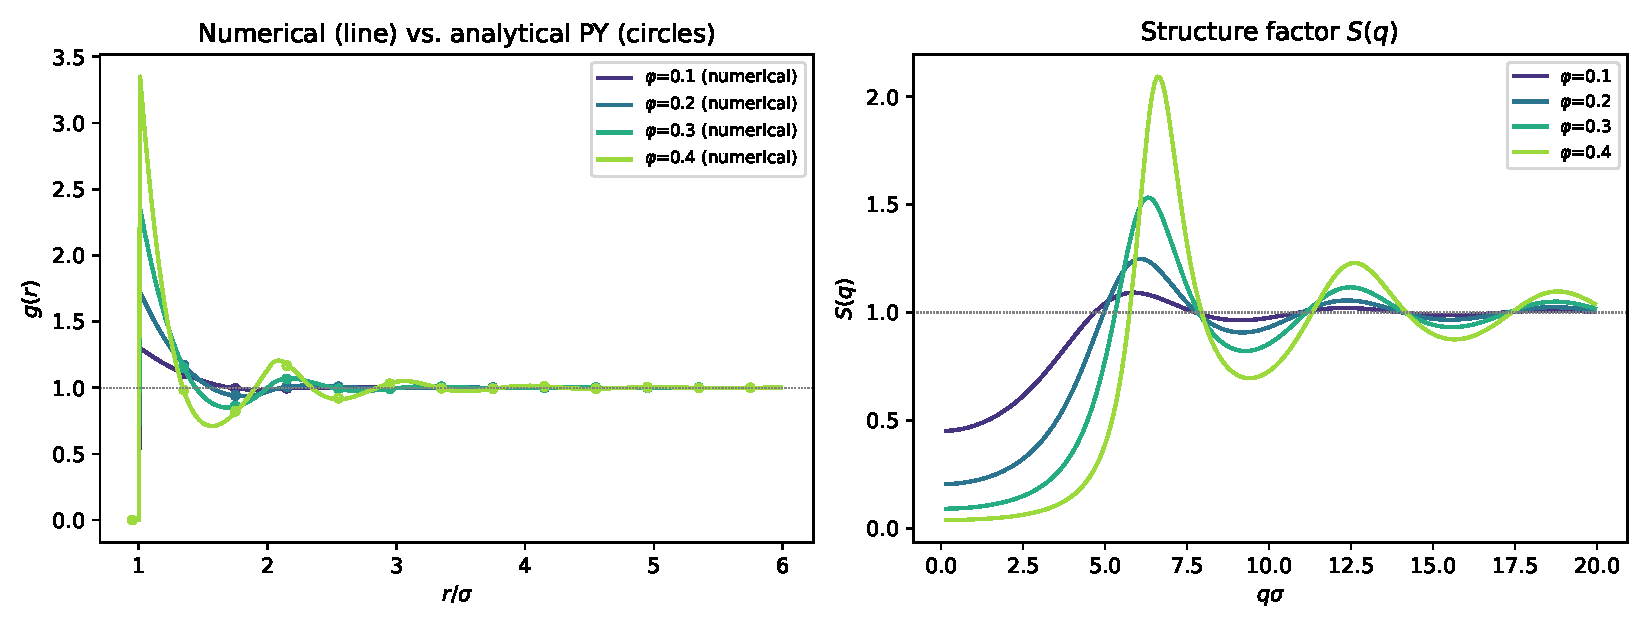
\includegraphics[width=\textwidth]{fig_hardsphere_validation.pdf}
\caption{$g(r)$ (left) and $S(q)$ (right) for hard spheres at
$\varphi\in\{0.1,0.2,0.3,0.4\}$: numerical solve (solid lines) vs.\ the exact
PY solution (open circles, sub-sampled for visibility).}
\label{fig:hs-validation}
\end{figure}

\subsection{Closure comparison at high density}

Figure~\ref{fig:closure-comparison} shows $g(r)$ for four different closures
applied to the same hard-sphere system at $\varphi=0.4$ (chosen because
closure differences are most visible near the freezing transition, where PY's
own known contact-value error becomes appreciable). PY and HNC bracket the
contact peak from below/above respectively (a well-known, textbook-level
result); Verlet and Duh--Haymet, both empirical-bridge-function closures, sit
between them and agree with each other almost exactly at this density.

\begin{figure}[h]
\centering
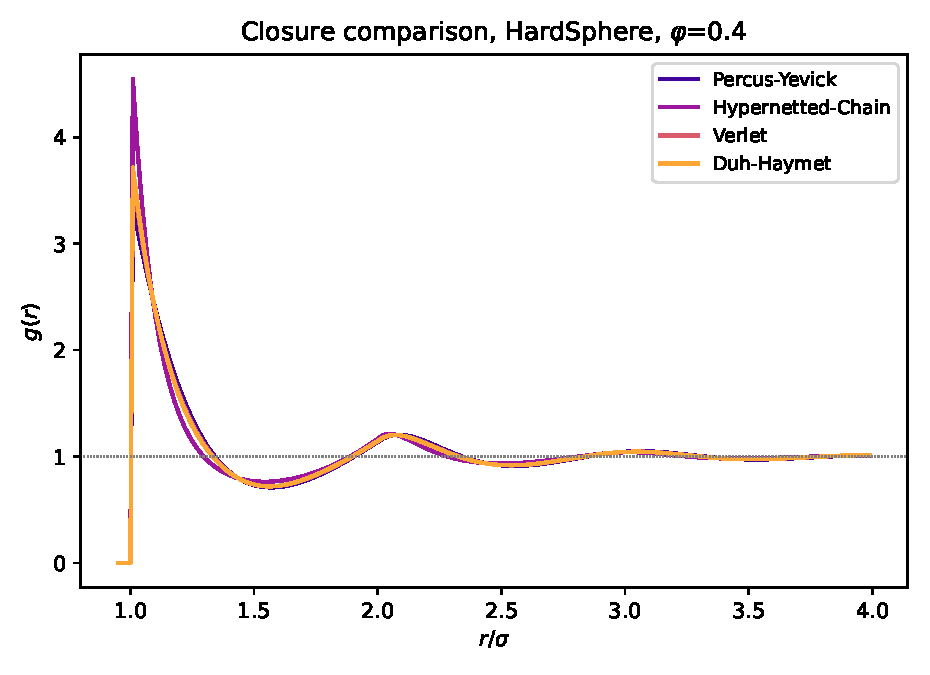
\includegraphics[width=0.75\textwidth]{fig_closure_comparison.pdf}
\caption{Closure comparison, hard spheres, $\varphi=0.4$.}
\label{fig:closure-comparison}
\end{figure}

\subsection{Charged systems: RMSA and the MSA contact-value problem}
\label{sec:critical-charged}

Plain MSA (Section~\ref{sec:closures}) can give an unphysical, negative
contact value $g(\sigma^+)<0$ for sufficiently strongly-coupled charged
systems --- a well-known limitation of MSA itself, not an artifact of this
implementation. Figure~\ref{fig:rmsa-hayter-penfold} shows a representative
$S(q)$ from the semi-analytical Hayter--Penfold RMSA solver
(Section~\ref{sec:hayter-penfold}), which sidesteps this issue by construction
via its own closed-form rescaling.

\begin{figure}[h]
\centering
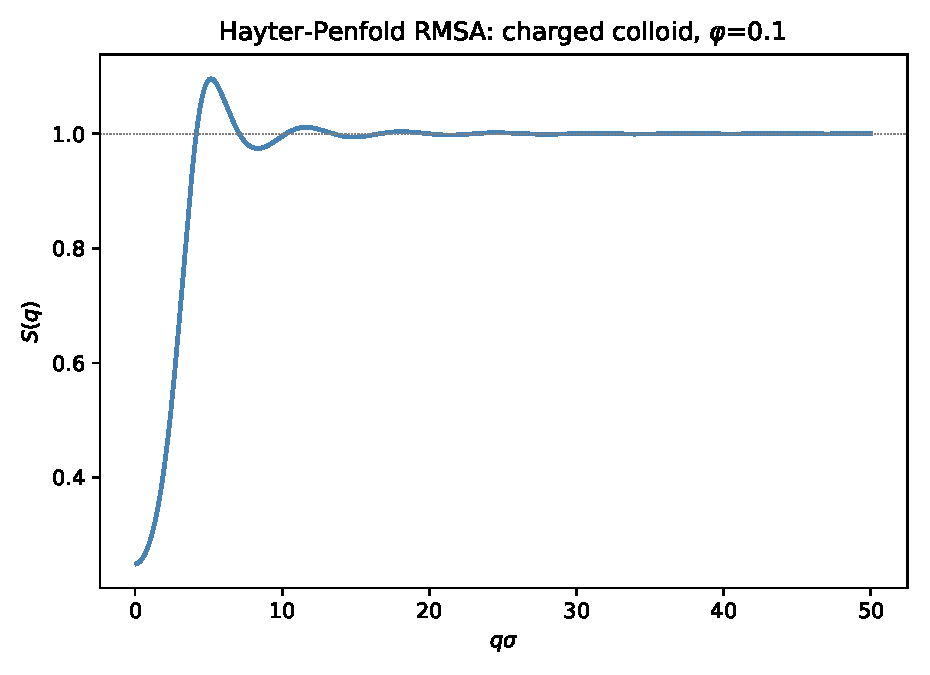
\includegraphics[width=0.7\textwidth]{fig_rmsa_hayter_penfold.pdf}
\caption{Hayter--Penfold RMSA structure factor for a charged colloid,
$\varphi=0.1$.}
\label{fig:rmsa-hayter-penfold}
\end{figure}

The general-potential numerical solver's own RMSA rescaling
(\code{OZsolver.solveRMSA()}, Section~\ref{sec:rmsa-closure}) implements the
same idea (extend the ``apparent'' hard-core radius outward until the contact
value there is non-negative) for arbitrary potentials, not just the
hard-core-Yukawa case Hayter--Penfold covers in closed form. This method was
found, on close comparison against \code{sasfit\_oz\_solver.c} itself, not to
be a plain bisection search at all: SASfit's own algorithm is a \emph{grow,
then bisect} scheme, where each solve's own full $g(r)$ array is scanned once
to see exactly how far the negative region extends (extending the excluded
region as far as that single solve's own data justifies, at no extra cost),
and only once a solve gives an already-non-negative result does it fall back
to bisecting the gap between the historical bounds. An earlier version of
this Python port used plain midpoint bisection instead, which was both less
efficient and, on inspection, genuinely buggy; it has since been rewritten to
match the C algorithm. \textbf{Three genuine bugs were found and fixed} in
total -- two in this Python port, one in SASfit's own C source:
\begin{enumerate}[nosep]
  \item \emph{Stale data on solver non-convergence} (Python port). Several
    solver classes (e.g.\ the \code{sundials4py}-based ones) simply print a
    message and return early when the underlying Newton--Krylov iteration
    fails to converge, without updating \code{self.radialDistributionFunction}
    -- meaning \code{getRDF()} silently returned data left over from
    whichever solve last actually succeeded, corrupting the search's own
    decisions and final result. Fixed with a solver-class-independent,
    Picard-iteration-based internal solve (\code{OZsolver.\_robustInlineSolve()}),
    warm-started between successive trials (the same density-continuation-
    with-warm-restarts principle already used for \code{solveEuRah()}'s own
    outer iteration).
  \item \emph{An off-by-one tautology in the original bisection-based port.}
    The old code's gate array, \code{gate4g[:mid+1]=0}, forced \code{g[mid]}
    to be exactly zero \emph{by construction} (it lies inside the assumed-
    excluded region) -- so checking \code{g[mid]} there could never
    distinguish anything. This is moot now that the port matches the actual
    C algorithm (which checks \code{g[igneg]}, the first point genuinely
    outside the current gate), but is recorded here since it was the first
    of the two Python-side bugs found.
  \item \emph{A genuine ambiguity in SASfit's own C source.} In the
    ``bisect'' branch (triggered once a trial gate already gives a
    non-negative result), the original C code computes a halved
    \code{indx\_max\_appearent\_sigma} but never resets \code{gate4g} between
    that smaller value and the previous trial boundary back to $1$, nor
    re-points its own scanning index (\code{igneg}) at the new boundary --
    so, taken literally, the next iteration's check and solve would silently
    re-test the same (larger) gate configuration rather than the smaller one
    the halving was meant to try. A related edge case (found only by testing
    this Python port directly): when the two search bounds are already
    adjacent integers, integer division always rounds down to the lower
    bound, which would discard a just-proven-sufficient upper bound and
    collapse the search straight back to no rescaling at all. Both were
    fixed identically in the Python port and in \code{sasfit\_oz\_solver.c}
    itself (the fix applied there is included in this project's own copy of
    the SASfit source, with a comment marking exactly what changed and why).
\end{enumerate}
With all three fixes applied, the algorithm reliably finds a small, sensible
rescaling and gives genuine, verified improvement over plain MSA on a
moderately-coupled test case (Figure~\ref{fig:msa-rmsa-rescue}: contact value
improves from $-0.132$ to $-0.053$, not perfectly zero but consistent with
finite grid resolution). A remaining open question, not yet resolved, is why
some more strongly-coupled cases still need an unexpectedly large
apparent-hard-core extension to reach a fully non-negative result --
plausibly a genuine slow-convergence issue in the underlying Picard iteration
at large gate sizes (a solver-reliability question, now clearly separated
from the algorithm's own correctness, which is independently validated
above), though this has not been fully resolved.

\begin{figure}[h]
\centering
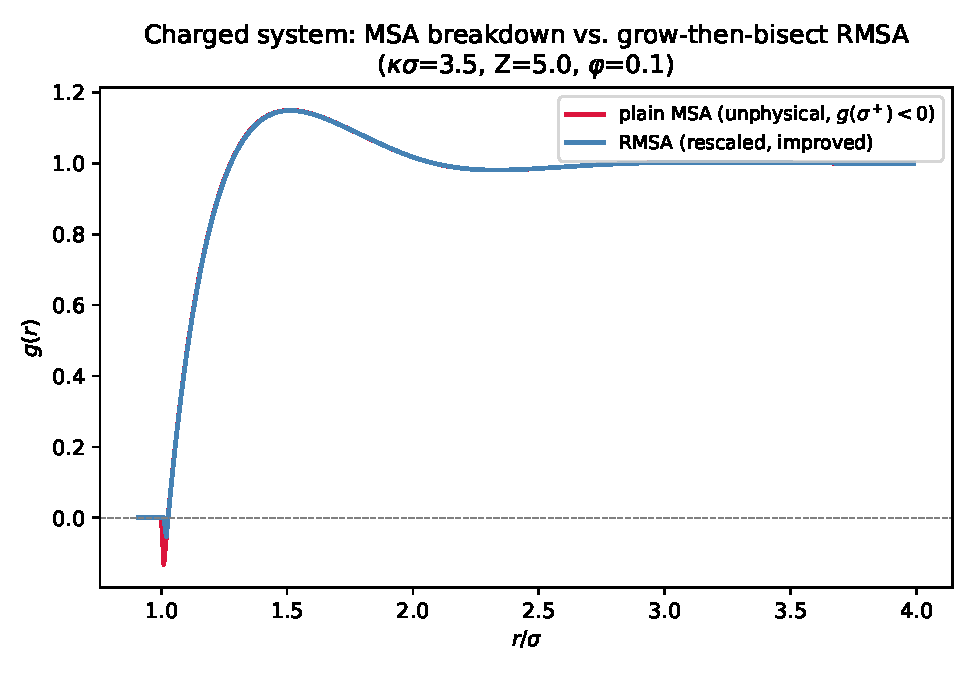
\includegraphics[width=0.7\textwidth]{fig_msa_rmsa_rescue.pdf}
\caption{Plain MSA's unphysical contact value vs.\ this project's own
grow-then-bisect RMSA rescue (post-fix), general-potential numerical solver,
DLVO potential, $\kappa\sigma=3.5$, $Z=5$, $\varphi=0.1$.}
\label{fig:msa-rmsa-rescue}
\end{figure}

\subsection{Behaviour near difficult/critical parameter regimes}
\label{sec:critical-params}

Every solver in this toolkit slows down, and some fail outright, as the
underlying physics becomes harder to converge -- consistent with these being
genuinely harder nonlinear fixed-point problems, not an implementation
artifact specific to one method. Three regimes recur throughout this
project's own testing history:
\begin{itemize}[nosep]
  \item \textbf{Dense hard spheres} ($\varphi\gtrsim0.45$, approaching random
    close packing): plain Picard iteration fails to converge outright; every
    accelerated method (Anderson, Biggs--Andrews order~$\ge$1, both
    Newton--Krylov families) still succeeds, but needs visibly more
    iterations/function evaluations than at moderate density.
  \item \textbf{Strongly-charged systems} (Section~\ref{sec:critical-charged}):
    plain MSA gives an unphysical negative contact value; the hand-written
    Anderson solver was found, in earlier testing, to converge to a
    \emph{silently wrong} answer on the hardest such case tried, without
    raising any error -- a more concerning failure mode than an honest
    non-convergence report, and a reminder to cross-check results from that
    solver specifically against an independently-validated one (e.g.\
    \code{sundials4py} GMRES) for difficult states.
  \item \textbf{Euler--Rahman (Section~\ref{sec:eurah})}: excluded entirely
    from this toolkit's offered closures, for the reasons documented there --
    a genuine exponential positive-feedback instability in the closure's own
    mathematical structure, not a solver-selection problem.
\end{itemize}
As a practical rule of thumb: if a solve fails to converge in one of these
regimes, trying a different solver algorithm first (Section~\ref{sec:solvers})
is more likely to help than increasing \code{maxIterations} on the same one,
since the empirical comparison of Section~\ref{sec:solver-comparison} shows
different algorithms fail on genuinely different subsets of hard cases.

\subsection{Speed}
\label{sec:speed-tests}

Figure~\ref{fig:solver-speed} times every solver on the same moderately-hard
case (hard spheres, $\varphi=0.4$, PY closure); Section~\ref{sec:solver-comparison}'s
own qualitative reliability comparison is the more important consideration in
practice, but at a given level of difficulty, the SUNDIALS KIN\_FP and GMRES
solvers are consistently among the fastest, followed by the hand-written
Anderson solver; plain Picard and Biggs--Andrews (order~0, equivalent to
Picard) are consistently the slowest, as expected of unaccelerated fixed-point
iteration.

\begin{figure}[h]
\centering
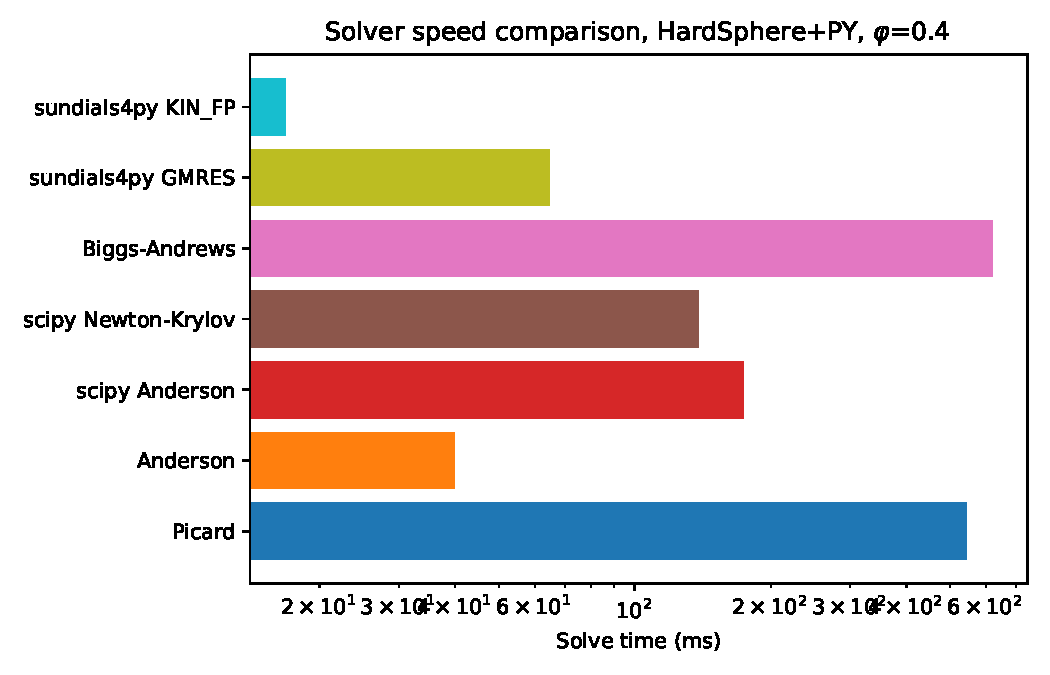
\includegraphics[width=0.85\textwidth]{fig_solver_speed.pdf}
\caption{Solve time by algorithm, hard spheres + PY, $\varphi=0.4$ (log scale).}
\label{fig:solver-speed}
\end{figure}

Separately, Figure~\ref{fig:grid-smoothness} revisits the grid-size question
of Section~\ref{sec:theory}: the relevant quantity for the underlying DST-based
Hankel transform's own speed is $N+1$, not $N$ itself, since the type-I DST
used here is equivalent to a real FFT of size $2(N+1)$. $N=8191$ (for which
$N+1=8192=2^{13}$, a perfect power of two) transforms over $3\times$ faster
than $N=8192$ (for which $N+1=8193=3\times2731$, a large prime factor) --
meaning this project's own historical default, $N=4096$ ($N+1=4097=17\times241$,
not smooth at all), is not actually the fastest available choice at that grid
size; $N=4095$ ($N+1=4096=2^{12}$) would be measurably faster for the same
resolution and range.

\begin{figure}[h]
\centering
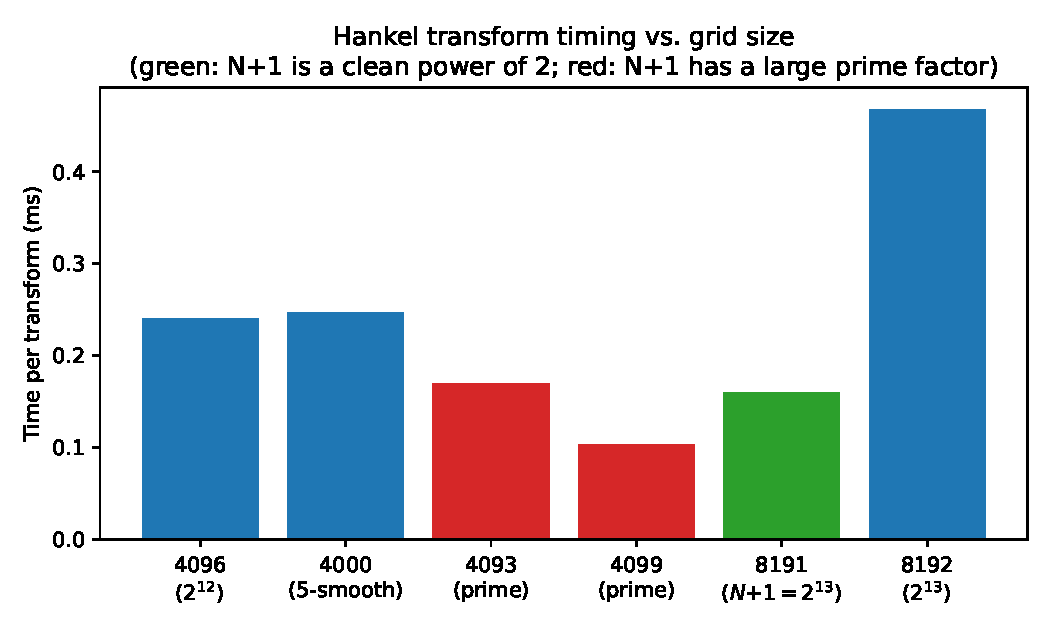
\includegraphics[width=0.85\textwidth]{fig_grid_smoothness.pdf}
\caption{Hankel transform timing vs.\ grid size $N$: the fastest and slowest
cases shown differ only in whether $N+1$ happens to be smooth, not in $N$'s
own magnitude or "niceness".}
\label{fig:grid-smoothness}
\end{figure}

\section*{Acknowledgements}
Formulas and algorithms throughout this document were ported directly from
SASfit's own source code (\code{src/sasfit\_oz/}, \code{src/plugins/*}), with
independent literature verification sought wherever practical.




\clearpage
\part{Multicomponent and polydisperse extension}







%======================================================================
\section{Scope and design constraint}

The starting point was that the existing solver stack is strictly
one-component: $c(r)$, $h(r)$ and $\gamma(r)$ are scalar arrays of length
$N_r$, and every closure in \code{update\_c} acts on them elementwise.

The design constraint adopted here was that \textbf{one-component behaviour
must remain bit-identical}. This is verifiable rather than aspirational: a
regression suite of eight potential/closure combinations is compared against
values recorded before the change (\S\ref{sec:regression}).

A second observation made the work far smaller than expected. Every solver
class --- Picard, the two Anderson variants, the two \code{scipy} solvers,
Biggs--Andrews and both SUNDIALS KINSOL drivers --- is \emph{already}
agnostic to the shape of the unknown. Searching the whole solver layer for
\code{numberOfRadialSamplingPoints} returns no hits: each iterates a flat
vector through \code{fixPointOperator} and never inspects what it represents.
Consequently the multicomponent problem can be carried through the existing
acceleration machinery unchanged, packed as the $p(p+1)/2$ unique pairs of the
symmetric $\Gamma_{ij}(r)$.

%======================================================================
\section{Multicomponent Ornstein--Zernike equations}

\subsection{Matrix form}

For $p$ species with number densities $\rho_i$, the OZ equations couple
$p(p+1)/2$ independent pair functions,
\begin{equation}
h_{ij}(r) = c_{ij}(r)
  + \sum_{\lambda=1}^{p}\rho_\lambda \int \mathrm{d}\mathbf{r}_1\,
    h_{i\lambda}(r_1)\,c_{\lambda j}(|\mathbf{r}-\mathbf{r}_1|).
\end{equation}
In Fourier space this becomes an algebraic matrix relation. With
$\mathsf{C}(q)$ the matrix of $\hat c_{ij}(q)$ and
$\boldsymbol{\rho}=\mathrm{diag}(\rho_i)$,
\begin{equation}
\mathsf{H}(q) = \bigl[\mathsf{I}-\mathsf{C}(q)\boldsymbol{\rho}\bigr]^{-1}
                \mathsf{C}(q),
\qquad
\mathsf{\Gamma}(q) = \mathsf{H}(q)-\mathsf{C}(q).
\label{eq:ozmatrix}
\end{equation}
The single scalar division of the one-component code,
$\hat\gamma = \hat c/(1-\rho\hat c) - \hat c$, is replaced by
\eqref{eq:ozmatrix}, solved as a small dense linear system at each of the
$N_r$ grid points. Nothing else in the fixpoint operator changes: the closure
step and the two Hankel transforms are the same operations applied to
$(p,p,N_r)$ arrays.

\subsection{Implementation}

The changes to \code{oZfixpointOperator.py} and \code{oZsolver.py} are:

\begin{itemize}[nosep]
\item the Hankel transforms act on the \emph{last} axis (\code{f.shape[-1]},
      \code{dst(...,\,axis=-1)}), which is identical for 1-D input but also
      accepts the pair-matrix arrays;
\item \code{isMulticomponent()}, \code{numberOfUniquePairs()},
      \code{packPairs()} and \code{unpackPairs()} convert between the
      symmetric $(p,p,N_r)$ matrix and the flat vector the solvers expect;
\item \code{fixPointOperatorForGammaMulticomponent()} implements
      \eqref{eq:ozmatrix};
\item \code{calculateSqMulticomponent()} and a multicomponent branch in
      \code{calculateRDF()} produce the observables;
\item \code{setStartValue()} accepts the longer vector.
\end{itemize}

\begin{remark}
Because every closure in \code{update\_c} is elementwise \code{numpy}, PY,
HNC, RY, HMSA, Verlet, BPGG and the rest all become multicomponent as soon as
the potential arrays carry pair indices. Closures requiring an auxiliary
reference solve (RHNC, MHNC, RMSA, EuRah) remain one-component, as do those
reading \code{repulsivePartOfP2Ppotential} (HMSA, VM, CJVM, BB, DH, CG,
SMSA), whose split arrays are still 1-D.
\end{remark}

\subsection{Public interface: 1-D curves preserved}

The public getters deliberately continue to return \emph{one}-dimensional
curves, so the plot tabs, \code{ozLib.solve()}'s curve dictionary and the
ASCII/CSV/Excel/clipboard exports need no modification:
\begin{align}
\code{getRDF()} &\;\rightarrow\; g_{NN}(r)=\sum_{ij}x_ix_j\,g_{ij}(r),\\
\code{getSq()}  &\;\rightarrow\; S^{M}(q) \text{ (the measured structure factor)}.
\end{align}
The full matrices are exposed alongside as
\code{partialRadialDistributionFunction} and
\code{partialStructureFactor}, both of shape $(p,p,N_r)$.

%======================================================================
\section{Structure-factor conventions}
\label{sec:conventions}

Three conventions appear in this problem and confusing them is an
order-of-magnitude error, so they are stated explicitly.

\paragraph{D'Aguanno--Klein (number-fraction) form.} Used internally by the
solver, following \cite{daguanno1991}:
\begin{equation}
S^{\mathrm{DAG}}_{ij}(q) = x_i\delta_{ij} + n\,x_i x_j\,\hat h_{ij}(q).
\end{equation}

\paragraph{Ashcroft--Langreth form.} Required by
\code{PolydisperseSASBase.I\_exact}, which builds
$G_i=F_i\sqrt{\rho_i}$ and contracts $G\mathsf{S}G$:
\begin{equation}
S^{\mathrm{AL}}_{ij}(q) = \delta_{ij} + \sqrt{\rho_i\rho_j}\,\hat h_{ij}(q).
\end{equation}

\paragraph{Conversion.} The two differ by a purely kinematic factor,
\begin{equation}
\boxed{\;S^{\mathrm{AL}}_{ij} = S^{\mathrm{DAG}}_{ij}\big/\sqrt{x_i x_j}\;}
\label{eq:alconv}
\end{equation}
which is easily checked on the diagonal: $S^{\mathrm{DAG}}_{ii}/x_i
= 1+n x_i \hat h_{ii} = S^{\mathrm{AL}}_{ii}$.

\paragraph{Measured structure factor.} What a scattering experiment sees,
weighted by the form amplitudes $b_i(q)$:
\begin{equation}
S^{M}(q) = \frac{\sum_{ij} b_i b_j S_{ij}(q)}{\sum_i x_i b_i^2},
\qquad
b_i(q)\propto \sigma_i^2\,\frac{j_1(q\sigma_i/2)}{q}.
\end{equation}

Conversion \eqref{eq:alconv} is applied in exactly one place in each module.
\S\ref{sec:traps} records two separate occasions on which omitting it caused
a silent factor-of-nine error.

%======================================================================
\section{Discretising a continuous size distribution}
\label{sec:moments}

\subsection{Moment matching}

A continuous distribution $F(\sigma)$ must be reduced to $p$ classes. The
naive choice of $p$ equally spaced diameters spanning
$\langle\sigma\rangle\pm3s$ is what the existing Robertus code uses. Following
\cite{daguanno1992} we instead impose
\begin{equation}
\sum_{i=1}^{p} x_i\,\sigma_i^{\,m} = \langle\sigma^m\rangle,
\qquad m=0,1,\dots,2p-1,
\label{eq:moments}
\end{equation}
i.e.\ $2p$ equations for the $2p$ unknowns $\{\sigma_i,x_i\}$. The Schulz
distribution is a gamma distribution, so \eqref{eq:moments} is precisely
Gauss--generalised-Laguerre quadrature: with $t=1/s^2-1$, the nodes and
weights of the weight function $x^{t}e^{-x}$ give
$\sigma_i = x_i^{\mathrm{node}}\langle\sigma\rangle/(t+1)$ directly. In Python
this is \code{scipy.special.roots\_genlaguerre}; in C,
\code{gsl\_integration\_fixed\_laguerre}.

\subsection{Verification}

For $s_\sigma=0.2$ and $p=3$ the classes are
$\sigma_i=\{0.7342,\,1.0532,\,1.4527\}$ with
$x_i=\{0.2795,\,0.6304,\,0.0901\}$, and the first $2p-1=5$ moments are
reproduced to eight decimal places (Table~\ref{tab:moments}).

\begin{table}[htbp]
\centering
\caption{Moments of the discrete three-class set against the continuous
Schulz distribution, $s_\sigma=0.2$. Exact through $m=2p-1=5$.}
\label{tab:moments}
\begin{tabular}{cccl}
\toprule
$m$ & discrete & Schulz & \\
\midrule
0 & 1.00000000 & 1.00000000 & exact \\
1 & 1.00000000 & 1.00000000 & exact \\
2 & 1.04000000 & 1.04000000 & exact \\
3 & 1.12320000 & 1.12320000 & exact \\
4 & 1.25798400 & 1.25798400 & exact \\
5 & 1.45926144 & 1.45926144 & exact \\
\bottomrule
\end{tabular}
\end{table}

\subsection{How many classes are needed?}

\cite{daguanno1992} report that $p=3$ is indistinguishable from $p=5$ up to
$s_\sigma=0.3$. This was reproduced independently
(Table~\ref{tab:pconv}): going from $p=1$ to $p=3$ changes $S^M$ by $0.54$,
whereas $p=3\rightarrow5$ changes it by $0.0015$. Polydispersity is therefore
a large effect that three moment-matched classes already capture.

\begin{table}[htbp]
\centering
\caption{Convergence in the number of classes. Polydisperse hard-core Yukawa,
$\langle\sigma\rangle=250$\,\AA, $Z=200$, $n^*=0.005$, $L_B=7.01$\,\AA,
$s_\sigma=0.2$, RY with $\alpha=0.5$.}
\label{tab:pconv}
\begin{tabular}{lcccc}
\toprule
 & $g_{NN}^{\max}$ & position & $S^{M}_{\max}$ & pairs \\
\midrule
$p=1$ (monodisperse) & 2.0375 & 6.06 & 2.0356 & 1 \\
$p=3$                & 1.7368 & 6.19 & 1.7478 & 6 \\
$p=5$                & 1.7340 & 6.19 & 1.7472 & 15 \\
\midrule
\multicolumn{5}{l}{$\max|g_{NN}(1)-g_{NN}(3)|=0.3583$,\quad
                   $\max|S^M(1)-S^M(3)|=0.5407$}\\
\multicolumn{5}{l}{$\max|g_{NN}(3)-g_{NN}(5)|=0.0115$,\quad
                   $\max|S^M(3)-S^M(5)|=0.0015$}\\
\bottomrule
\end{tabular}
\end{table}

The peak sits at $r\approx6.2\langle\sigma\rangle$ against a mean spacing
$n^{-1/3}=5.85\langle\sigma\rangle$, as expected for a strongly correlated
charged system.

\begin{remark}
The moment-matching method transfers to the adhesive-sphere model, and would
let the Robertus plugin use fewer classes for the same accuracy. The specific
claim ``$p=3$ suffices'' does \emph{not} transfer: it was established for
RY--Yukawa against Monte Carlo, and sticky spheres are far more sensitive to
the contact region.
\end{remark}

%======================================================================
\section{Polydisperse hard-core Yukawa}

\subsection{Charge-parameterised form}

Following \cite{daguanno1992}, the pair potential is
\begin{equation}
\beta\varphi_{ij}(r) = A_iA_j\,\frac{e^{-\kappa r}}{r},\qquad r>\sigma_{ij},
\qquad
A_i = Z_i\sqrt{L_B}\,\frac{e^{\kappa\sigma_i/2}}{1+\kappa\sigma_i/2},
\label{eq:dkpot}
\end{equation}
with a hard core at $\sigma_{ij}=(\sigma_i+\sigma_j)/2$. The amplitude
\emph{factorises per species}, because
$\exp(\kappa\sigma_{ij}) = \exp(\kappa\sigma_i/2)\exp(\kappa\sigma_j/2)$;
this is what allows the $A_iA_j$ form.

\paragraph{Screening.} $\kappa$ is the inverse Debye length due to the
\emph{small ions}. For a salt-free suspension with monovalent counterions,
charge neutrality gives $n_{\text{counter}}=\sum_i n_iZ_i$ and hence
\begin{equation}
\kappa^2 = 4\pi L_B\sum_i n_i Z_i
\label{eq:kappa}
\end{equation}
--- the \emph{first} power of $Z$. Using $Z^2$ produces a near-ideal-gas
$S(q)$ (see \S\ref{sec:traps}).

\subsection{Size dependence of the charge}
\label{sec:charge}

How the valence scales with size is genuinely unsettled, so it is a user
input rather than a constant. \cite{daguanno1991} assume constant surface
charge density, $Z\propto\sigma^2$, and explicitly flag it as having ``little
precise experimental information''. Charge-renormalisation saturation
(Alexander \emph{et al.}) and electrophoresis on highly charged low-salt
spheres both indicate $Z\propto\sigma$ instead. Three routes are provided:

\begin{center}
\begin{tabular}{@{}p{0.30\textwidth}p{0.62\textwidth}@{}}
\toprule
\code{chargeExponent} & $Z_i = Z_{\text{ref}}(\sigma_i/\langle\sigma\rangle)^n$;
  $n=2$ constant surface charge density (default), $n=1$ linear in size,
  $n=0$ size-independent \\
\code{componentValences} & explicit per-component array, overrides the power law \\
\code{screeningValences} & a \emph{different} charge for $\kappa$, so screening
  may use the bare charge while the amplitude uses the effective one \\
\bottomrule
\end{tabular}
\end{center}

The default $n=2$ exists only so that published D'Aguanno--Klein setups
reproduce; it is not a recommendation. Charge renormalisation is deliberately
\emph{not} implemented: its definition for a polydisperse system is unsettled
(even for one component the Alexander edge-linearisation $Z_{\text{eff}}$ and
the extrapolated point charge $Q_{\text{eff}}$ disagree), and embedding one
choice inside a fitting routine would hide a contested assumption.

\paragraph{Magnitude of the effect.} Table~\ref{tab:charge} shows the choice
is comparable in size to the polydispersity effect itself, so it is not a
detail. Note also that $\alpha$-scaling and screening are coupled through
\eqref{eq:kappa}: changing the exponent moves both the amplitude prefactor
and the screening length unless \code{screeningValences} decouples them.

\begin{table}[htbp]
\centering
\caption{Effect of the charge-scaling exponent. $p=3$, $s_\sigma=0.2$,
D'Aguanno--Klein parameters, RY $\alpha=0.5$.}
\label{tab:charge}
\begin{tabular}{lcccc}
\toprule
scaling & $Z_i$ & $\kappa$ & $g_{NN}^{\max}$ & $S^M_{\max}$\\
\midrule
$n=2$ (default) & 107.8 / 221.8 / 422.0 & 0.6054 & 1.7368 & 1.7478\\
$n=1$           & 146.8 / 210.6 / 290.5 & 0.5936 & 1.9262 & 1.8381\\
$n=0$           & 200 / 200 / 200        & 0.5936 & 2.0384 & 1.7724\\
\bottomrule
\end{tabular}
\end{table}

An internal consistency check falls out of \eqref{eq:kappa}: $n=0$ and $n=1$
must share a $\kappa$, because $\sum_i x_i\sigma_i=\langle\sigma\rangle=1$ by
construction, while $n=2$ raises it by exactly
$\sqrt{\langle\sigma^2\rangle}=\sqrt{1.04}=1.0198$. Both hold to four
decimals.

\subsection{MSA-consistent \texorpdfstring{$(z,K)$}{(z,K)} form}
\label{sec:zk}

For direct comparison with the analytic MSA/RMSA path the same convention
must be used. From the polydisperse Yukawa specification,
\begin{equation}
c_{ij}(r) = K_{ij}\,\frac{e^{-z(r-\sigma_{ij})}}{r},\quad r>\sigma_{ij},
\qquad K_{ij}=K\,\delta_i\delta_j,
\qquad \delta_i = d_i\,e^{-z\sigma_i/2},
\label{eq:msapot}
\end{equation}
with $g_{ij}(r)=0$ for $r\le\sigma_{ij}$. MSA sets $c=-\beta U$, so
\begin{equation}
\beta U_{ij}(r) = -K\,\delta_i\delta_j\,\frac{e^{-z(r-\sigma_{ij})}}{r},
\end{equation}
i.e.\ \textbf{$K>0$ is attractive and $K<0$ repulsive}, and there is
\emph{no} $\sigma_{ij}$ prefactor. Note that
\code{PolydisperseOneYukawaMSA} takes $\delta_i$ \emph{directly} --- its
default \code{np.ones(N)} means $\delta_i=1$, not $d_i=1$ --- so the
exponential in \eqref{eq:msapot} must not be applied a second time
(\S\ref{sec:traps}, item 9).

%======================================================================
\section{Rogers--Young for mixtures}

\subsection{Closure}

The RY closure is applied pairwise with a \emph{single shared} mixing
function --- there is no $ij$ subscript on $f$ in \cite{daguanno1991}:
\begin{equation}
h_{ij}(r) = -1 + e^{-\beta\varphi_{ij}(r)}
  \left[1+\frac{e^{f(r)\gamma_{ij}(r)}-1}{f(r)}\right],
\qquad
f(r) = 1-e^{-\alpha r},
\label{eq:ry}
\end{equation}
interpolating between PY ($\alpha\to0$) and HNC ($\alpha\to\infty$).

\subsection{Thermodynamic consistency fixes \texorpdfstring{$\alpha$}{alpha}}
\label{sec:alpha}

$\alpha$ is not a free parameter: it is determined by requiring the
compressibility and virial routes to the pressure to agree. For a mixture this
is a \emph{scalar} condition --- which sidesteps the apparent difficulty that
a mixture has a full compressibility \emph{matrix}:
\begin{align}
\chi^{-1}_{\text{comp}} &= 1 - n\sum_{ij}x_ix_j\,\hat c_{ij}(0),
\label{eq:chicomp}\\
\chi^{-1}_{\text{vir}} &= \frac{\partial(\beta P)}{\partial n},
\label{eq:chivir}
\end{align}
with the virial pressure
\begin{equation}
\frac{\beta P}{n} = 1
  + \frac{2\pi}{3}n\sum_{ij}x_ix_j\sigma_{ij}^3 g_{ij}(\sigma_{ij}^+)
  - \frac{2\pi}{3}n\sum_{ij}x_ix_j\int r^3 g_{ij}(r)\,
    \bigl(\beta U_{ij}\bigr)'(r)\,\mathrm{d}r .
\label{eq:virial}
\end{equation}

\paragraph{The contact term.} \cite{daguanno1991}'s equation for $\beta P$
omits the second term of \eqref{eq:virial}, legitimately, because their
macroions are so strongly charged that $g_{ij}(\sigma_{ij}^+)\approx0$. That
is \emph{not} safe in general: this model has a genuine hard core and $K$ may
be small, so contact is reachable and the term is first order in the
pressure. It is included here, with $g_{ij}$ at contact obtained by linear
extrapolation from the first two grid points outside $\sigma_{ij}$. This
extrapolation is the least certain step in the whole search and is flagged as
such in the code.

\paragraph{Numerics.} Two traps, both encountered:
\begin{enumerate}[nosep]
\item the \textbf{pair potential must be held fixed} while $n$ is perturbed.
      In the charge-parameterised form \eqref{eq:dkpot} $\kappa$ depends on
      the counterion density, so rebuilding the system at $n\pm\Delta n$
      differentiates a density-dependent potential; the symptom is a residual
      stuck near $+65$ that never crosses zero. In the $(z,K)$ form
      \eqref{eq:msapot} the potential is density-independent and the problem
      does not arise.
\item \textbf{cold-start each $\alpha$}. Warm-starting across qualitatively
      different $\alpha$ destabilises the search; warm-starting across the
      $n\pm\Delta n$ perturbations is fine, and is what \cite{daguanno1991}
      do, holding $\alpha$ fixed there because it varies slowly with $n$.
\end{enumerate}

\paragraph{Result.} At $\varphi=0.2$, $K=0$, $z=2$ with three classes the
search returns $\alpha=0.2166$ with residual $1.2\times10^{-5}$ --- a clean
root, and a plausible hard-sphere value. The residual is monotone in
$\alpha$ (Table~\ref{tab:alpha}).

\begin{table}[htbp]
\centering
\caption{Thermodynamic inconsistency
$\chi^{-1}_{\text{comp}}-\chi^{-1}_{\text{vir}}$ versus $\alpha$;
$\varphi=0.2$, $z=2$, $p=3$.}
\label{tab:alpha}
\begin{tabular}{lcccc}
\toprule
$\alpha$ & 0.20 & 0.50 & 1.00 & 2.00\\
\midrule
$K=0$   & $+0.0127$ & $-0.1847$ & $-0.4002$ & $-0.6054$\\
$K=0.5$ & $-0.2219$ & $-0.3012$ & $-0.3881$ & $-0.4697$\\
\bottomrule
\end{tabular}
\end{table}

\begin{remark}[A consistent $\alpha$ need not exist]
For $K=0.5$ the residual is negative across the whole bracket: no $\alpha$
makes the two routes agree. The implementation returns the closest endpoint
and reports ``no consistent alpha found'' rather than presenting it as a
solution. This is a property of the closure, not a numerical failure.
\end{remark}

\subsection{Validation against the literature}

The one-component limit reproduces Table~1 of \cite{daguanno1991}
(their test~3: $\beta\varphi(x)=(1000/x)e^{-0.95x}$, $n\sigma^3=0.01432$).
The self-consistent $\alpha=0.3942$ gives Table~\ref{tab:dk}.

\begin{table}[htbp]
\centering
\caption{One-component RY against \cite{daguanno1991} Table~1, test~3.}
\label{tab:dk}
\begin{tabular}{lrrr}
\toprule
quantity & this work & D'Aguanno--Klein & deviation\\
\midrule
$1/S(0)$   & 93.787 & 93.80 & $0.01\%$\\
$P^{ex}$   & 36.458 & 36.45 & $0.02\%$\\
$U^{ex}$   & 20.145 & 20.09 & $0.27\%$\\
$g_{\max}$ &  2.069 &  2.08 & $0.54\%$\\
\bottomrule
\end{tabular}
\end{table}

The two quantities that \emph{enter} the consistency condition agree to
$0.01$--$0.02\%$, which is the sharpest available test. Two further checks:
\begin{itemize}[nosep]
\item \textbf{HNC limit.} At large $\alpha$ the solver gives
      $g_{\max}=1.937$, $1/S(0)=77.69$, $U^{ex}=20.56$, $P^{ex}=36.94$
      against the paper's HNC column $1.94$, $77.5$, $20.57$, $36.95$ ---
      three-digit agreement, an independent check on the closure and the
      transforms.
\item \textbf{Grid insensitivity.} Results are flat to four decimal places
      from 50 to 400 points per $\sigma$; only $1/S(0)$ shifts slightly with
      $r_{\max}$ through the $q\to0$ extrapolation. Neither paper specifies
      its grid, and the residual differences in $g_{\max}$/$U^{ex}$ are
      therefore attributable to their (unreported) $\alpha$ or $\Delta n$
      rather than to discretisation.
\end{itemize}

\subsection{Cross-validation against the analytic MSA path}

Because RY and MSA both set $c=-\beta U$ outside the core, the
\emph{derivative} $\mathrm{d}S/\mathrm{d}K$ at $K\to0$ must agree even though
the closures differ. This is the decisive test of the potential convention of
\S\ref{sec:zk}, and it is what exposed the $\delta_i$ double-counting bug.
Table~\ref{tab:msary} shows agreement after the fix.

\begin{table}[htbp]
\centering
\caption{$\mathrm{d}S_{NN}/\mathrm{d}K$ at $Q=0.5$, $z=2$, three classes.
Agreement is near-exact where both closures reduce to the same physics and
degrades with density where PY and RY genuinely differ.}
\label{tab:msary}
\begin{tabular}{lccc}
\toprule
$\varphi$ & MSA & RY & ratio\\
\midrule
0.002 & 0.03031 & 0.03085 & 1.018\\
0.020 & 0.24025 & 0.24900 & 1.036\\
0.100 & 0.41790 & 0.47266 & 1.131\\
\bottomrule
\end{tabular}
\end{table}

Before the fix the ratio was $0.14$ at all three densities, consistent with
$1/e^{-z\sigma/2}\,^2=1/0.135=7.4$.

%======================================================================
\section{Solver strategy}
\label{mc:sec:solvers}

Three tiers are tried in order, fastest first, each strictly more robust than
the previous one.

\paragraph{Tier 1 --- Anderson (\code{KIN\_FP}) with Picard
pre-conditioning.} Fastest where it works. Anderson diverges from a cold
start on this problem: a hand-written implementation was \emph{slower} than
undamped Picard when damped enough to be stable (851 versus 677 iterations)
and diverged otherwise, and SUNDIALS' \code{KIN\_FP} diverged too, damped or
not. The remedy is a short run of plain undamped Picard --- which \emph{is}
contractive here --- before handing over. Measured: 0 pre-steps diverges, 20
already works, 40 is the time optimum; 50 is the default for margin.

\paragraph{Tier 2 --- Newton--Krylov (GMRES with \code{KIN\_LINESEARCH}).}
A different algorithm, not a variant: damped Newton steps on the residual
$F(u)=G(u)-u$ with the Jacobian applied matrix-free through GMRES. It
converged in \emph{every} regime tried, in a strikingly constant 31--40
Newton iterations regardless of difficulty --- the signature of global
convergence via linesearch. The cost is wall-clock: each Newton step requires
many GMRES inner iterations, each a full function evaluation, so it runs
3--6$\times$ slower than Anderson where Anderson works.

Tuning follows SASfit's own \code{KIN\_sasfit\_configure()}:
\code{MaxNewtonStep}$=100n$ (not $n$), \code{FuncNormTol}$=10^{-10}$ and
\code{ScaledStepTol}$=10^{-13}$ (deliberately different from each other),
\code{MaxRestarts}$=10$, \code{ETACHOICE1}.

\paragraph{Tier 3 --- Picard}, undamped then progressively damped.

\paragraph{The Python side.} \code{sundials4py} is available as a prebuilt
wheel on PyPI (version 7.8.0), so no binding generation or C++ build is
needed. Measured on the same problem, KIN\_FP is the best of the Python
solvers on every count: it agrees with the others where they converge, is
2--4$\times$ faster, and on the hard state point it fails to converge in
0.9\,s rather than converging onto a spurious root.

\begin{center}
\begin{tabular}{lccc}
\toprule
state point & KIN\_FP & \code{scipy} Anderson & Picard\\
\midrule
$\varphi=0.02$, $K=1$ & \textbf{0.1\,s} & 0.2\,s & 0.1\,s\\
$\varphi=0.1$, $K=0.2$ & \textbf{0.2\,s} & 0.8\,s & ---\\
$\varphi=0.1$, $K=1$ & rejected, 0.9\,s & rejected, 5.6\,s & diverged, 56\,s\\
\bottomrule
\end{tabular}
\end{center}

A caution recorded earlier in this project --- that
\code{sundials4py} might silently ignore \code{KINSetMAA} when it is called
after \code{KINInit}, as pyozGUI does --- was \emph{tested and found to be
unfounded}. On a deliberately slow linear fixed point, MAA${}=0$ took 757
iterations and MAA${}=5$ took 93, \emph{identical in both call orders}, so
Anderson acceleration is genuinely active. The C requirement is nonetheless
real: calling \code{KINSetMAA} after \code{KINInit} segfaults on SUNDIALS
7.1.1, so the C core keeps the documented order.

\begin{table}[htbp]
\centering
\caption{Solver tier actually used, and wall-clock time, across seven
parameter regimes (C implementation, SUNDIALS~7, $N_r=4095$).}
\label{tab:tiers}
\begin{tabular}{lcc}
\toprule
regime & time & tier\\
\midrule
$p=3$, $s=0.2$              & 0.25\,s & Anderson\\
$p=1$ monodisperse          & 0.03\,s & Anderson\\
$p=5$, $s=0.3$              & 6.85\,s & Newton--Krylov\\
$p=3$, $s=0.4$              & 0.32\,s & Anderson\\
$p=3$, $s=0.2$, $5\times$ density   & 0.29\,s & Anderson\\
$p=3$, $s=0.2$, $0.2\times$ density & 0.25\,s & Anderson\\
$p=7$, $s=0.25$             & 4.11\,s & Anderson\\
\bottomrule
\end{tabular}
\end{table}

\paragraph{Never trust the convergence flag.} \code{KINSol} can return
\code{KIN\_SUCCESS} after diverging: once the RY closure's exponent clipping
pins values near $10^{217}$ the internal stopping test is defeated. This was
observed at $p=5$, $s_\sigma=0.3$, where $S^M$ was returned as
$\sim10^{222}$ \emph{with a success flag}. Both KINSOL drivers therefore
recompute the residual after \code{KINSol} returns and reject the result
unless it really is small. With that check in place the regime correctly falls
through to Newton--Krylov and returns the right answer.

%======================================================================
\section{The SASfit plugin}

The C implementation is shipped as
\code{src/plugins/ry\_polydisperse\_yukawa/}, exporting
\code{sasfit\_sq\_RYPolydisperseYukawa}. It follows the established plugin
conventions: \code{sasfit\_cmake\_plugin()}, \code{include/private.h}, Doxygen
\code{\textbackslash defgroup}/\code{\textbackslash ingroup} with an HTML
parameter table, \code{SASFIT\_PLUGIN\_EXP\_*} registration, and the
\code{func}/\code{\_f}/\code{\_v} triad with \code{\_f} and \code{\_v} stubbed
to $0$ as in SASfit's own \code{sq\_*} plugins.

\paragraph{Transform.} The radial transform is a DST-I built from a radix-2
real FFT, which is why $N_r+1$ must be a power of two; $N_r=2^{12}-1$ at 100
points per $\sigma$ matches the Python grid exactly. The DST-I agrees with
\code{scipy.fft.dst(type=1)} exactly.

\paragraph{Caching.} A solve costs a few tenths of a second, so re-solving per
$q$-point would make any scan or fit unusable. The solved system is cached on
the full parameter set and successive solves warm-start from the previous
$\gamma$; 2000 further $q$-points after the first cost effectively nothing.

\paragraph{Portability.} Builds and runs against both SUNDIALS~7.1.1 and
6.4.1 with identical results (v7 about 30\% faster). The one relevant API
break is \code{SUNContext\_Create}, whose first argument became a typed
\code{SUNComm} with a \code{SUN\_COMM\_NULL} sentinel in v7; this is handled
by a macro switched on \code{SUNDIALS\_VERSION\_MAJOR}. Version~7 also
requires \code{-lsundials\_core}, which does not exist in v6.

\paragraph{Performance history.} Four measured steps, each kept as a test:

\begin{center}
\begin{tabular}{lr}
\toprule
change & time\\
\midrule
initial (GSL \code{LU\_decomp} per $q$-point, damped Picard) & 15.1\,s\\
inline small-matrix solve + upper-triangle symmetry          & 8.3\,s\\
undamped Picard                                              & 2.3\,s\\
Anderson (\code{KIN\_FP}) + Picard pre-conditioning          & \textbf{0.26\,s}\\
\bottomrule
\end{tabular}
\end{center}

The first version was \emph{slower than \code{numpy}}, because it performed
3.4 million GSL $3\times3$ \code{LU\_decomp} calls, where GSL's generality
dominates the actual arithmetic.

\paragraph{Agreement with Python.} The full $S^M(q)$ curve matches the Python
implementation to $7.1\times10^{-11}$ relative on the Picard path and
$1.3\times10^{-8}$ on the Anderson path (the latter being the solver
tolerance, not an error).

\paragraph{$\alpha$ in the plugin.} The consistency search costs three extra
OZ solves per trial value and is far too slow inside a fit. The plugin
therefore takes $\alpha$ as a parameter; it should be determined once in the
GUI (\S\ref{sec:alpha}) and then held fixed, which is justified because
$\alpha$ varies slowly with density --- the same reasoning
\cite{daguanno1991} use when holding it constant across their own
finite-difference density derivative.

%======================================================================
\section{New GUI tabs}

\code{oZgui.py} gained a top-level notebook and an \code{\_addExtraTabs()}
hook driven by a registry,
\begin{lstlisting}[basicstyle=\ttfamily\footnotesize]
EXTRA_TABS = [
    ("polydisperse_yukawa_tab",     "PolydisperseYukawaTab",     "Polydisperse Yukawa"),
    ("robertus_shs_tab",            "RobertusSHSTab",            "Robertus SHS"),
    ("ry_polydisperse_yukawa_tab",  "RYPolydisperseYukawaTab",   "RY Polydisperse Yukawa"),
]
\end{lstlisting}
Each tab is a self-contained \code{ttk.Frame} isolated by \code{try/except},
so adding one is a single line and an import failure costs only that tab.

Both new tabs follow the same pattern: a parameter panel; plot tabs for
$I(Q)$, the approximation error, $S_{ij}(Q)$, $S(Q)$ and the size
distribution; a Summary tab; a threaded compute handing results back through a
queue (Tk is not thread-safe); and ASCII/CSV export.

\paragraph{Approximation schemes.} Because both new SAS classes derive from
the same \code{PolydisperseSASBase}, all six of SASfit's schemes for combining
a structure factor with a size distribution --- monodisperse, decoupling
(Kotlarchyk--Chen), local monodisperse (Pedersen), partial structure factors,
scaling (Gazzillo) and van der Waals one-fluid --- come for free, and the
error of each can be read directly off the plot. The approximation code is
byte-identical between the tabs, so comparing them is a genuine test of how
those approximations fare for a different interaction rather than a comparison
of two implementations.

\paragraph{Failure reporting.} An individual scheme that fails does not lose
the run: it is marked ``unavailable'' in the summary. This matters because the
\emph{monodisperse} reference can have no PY solution at a state point where
the polydisperse system does. Adhesive-sphere failures are additionally
translated into actionable advice --- \emph{increase} $\tau$, since smaller
$\tau$ is stickier and below $\tau_c(\varphi)$ the adhesive PY closure has no
physical solution at all.

\paragraph{$\alpha$ is not exposed.} Following \S\ref{sec:alpha}, the RY tab
has no $\alpha$ entry field. It is solved for on every Compute and reported in
the Summary, together with the residual and an explicit warning when no
consistent value exists.


%======================================================================
\section{Generic polydisperse models: any potential, any closure}
\label{sec:generic}

The multicomponent machinery of \S\ref{sec:conventions} was initially reached
only through one bespoke potential. This section describes its generalisation
to \emph{any} of the library's eighteen one-component potentials, combined
with any closure that works multicomponent and any form factor.

\subsection{Reusing eighteen setters unmodified}

The potentials are not rewritten. \code{getrArray()} gains an override; the
builder points it at $r/\sigma_{ij}$ and calls the ordinary one-component
setter. Because every setter measures its hard core against
\code{hardSphereDiameter}, which is unity in those reduced units, that core
lands exactly at $\sigma_{ij}$ while the tail is evaluated at the reduced
separation. The mixing rule is therefore
\begin{equation}
\sigma_{ij}=\tfrac12(\sigma_i+\sigma_j),
\qquad
u_{ij}(r) = u\!\left(r/\sigma_{ij}\right),
\label{eq:reducedtail}
\end{equation}
i.e.\ every pair sees the same interaction \emph{shape} in units of its own
contact distance. This is the assumption Robertus \emph{et al.}\ make for
size-independent stickiness, and it is what makes the construction
potential-agnostic: $\varepsilon$, $\delta$, $n$, $\tau$ keep their
reduced-unit meaning for every pair, so no per-potential mixing rule need be
invented.

\begin{remark}
Equation \eqref{eq:reducedtail} is a modelling choice, not a derivation. For
Lennard-Jones the conventional alternative is Lorentz--Berthelot,
$\varepsilon_{ij}=\sqrt{\varepsilon_i\varepsilon_j}$ with per-species
$\varepsilon$; that is a different model and would require per-species tail
parameters, which the builder deliberately does not invent.
\end{remark}

\paragraph{Charge-coupled potentials are refused.} DLVO, DLVO-Hydra,
IonicMicrogel and the dedicated polydisperse Yukawa have amplitudes that scale
with particle size and a $\kappa$ set by the whole distribution through the
counterion density \eqref{eq:kappa}. The reduced-tail rule is simply wrong for
them, so they are rejected with a message rather than silently mis-modelled.

\paragraph{Verification.} With $s_\sigma=0$ and one class the generic path
reproduces the ordinary one-component setters \textbf{bit-identically}
(maximum difference $0.00\times10^{0}$ for hard spheres, square well and
Lennard-Jones; the first and third reproduce the recorded values $2.3561180274$
and $2.1635946756$). This is the sharpest available check that the
generalisation leaves validated physics untouched.

\subsection{Quadrature rule per distribution}
\label{sec:nodes}

All four supported distributions (Schulz, Gaussian, log-normal, Weibull) have
\emph{analytic} moments, so computing $\langle\sigma^n\rangle$ is never the
difficulty. The difficulty is the map from moments to nodes: the Golub--Welsch
Hankel eigenproblem is classically ill-conditioned even with exact input.

\begin{table}[htbp]
\centering
\caption{Condition number of the log-normal Hankel matrix built from exact
moments. Double precision carries about $10^{16}$; past that Cholesky does
\emph{not} fail, it silently returns nonsense.}
\begin{tabular}{lccc}
\toprule
 & $s=0.3$ & $s=0.4$ & $s=0.5$\\
\midrule
$N=6$  & $1.6\times10^{7}$  & $1.7\times10^{7}$  & $1.2\times10^{8}$\\
$N=8$  & $2.1\times10^{10}$ & $1.9\times10^{11}$ & $4.7\times10^{13}$\\
$N=10$ & $7.0\times10^{13}$ & $1.7\times10^{16}$ & $5.4\times10^{19}$\\
$N=12$ & $6.4\times10^{17}$ & $1.2\times10^{21}$ & $2.3\times10^{27}$\\
\bottomrule
\end{tabular}
\end{table}

A closed-form classical rule is therefore used wherever one exists, bypassing
the Hankel step entirely: generalised Gauss--Laguerre for the Schulz/gamma
weight and Gauss--Hermite for the Gaussian, both stable in double precision;
Golub--Welsch with 200-digit arithmetic only for log-normal and Weibull, which
have no classical rule. All four are moment-exact to $\sim10^{-16}$.

\paragraph{A physical guard on the Gaussian.} Gauss--Hermite places its
outermost node at $u\approx\pm2.86$, so $\sigma$ reaches zero near
$s\approx0.35$. A form factor tolerates a vanishing bin; a structure factor
does not, because a hard core must be placed at every $\sigma_{ij}$. Nodes
below $10^{-3}\langle\sigma\rangle$ are dropped and the weights renormalised
--- sacrificing moment-exactness rather than physicality. The test is
deliberately \emph{relative}: at $s=0.35$ the node sits at $10^{-4}$, positive
but still a zero-diameter particle, so a bare $\sigma>0$ check is insufficient.

\subsection{Structure factor and form factor need different resolutions}
\label{sec:nff}

The two averages behave differently in $\sigma$. $S_{ij}(Q)$ varies smoothly
with size, so three to five moment-matched classes suffice --- and the solve
costs $O(p^2)$ pair transforms, so $p$ should stay small. The form-factor
average $\langle|F|^2\rangle$ oscillates: at high $Q$ the phase $QR$ spans
about $Q\langle\sigma\rangle s_\sigma$ radians across the distribution. The
two class counts are therefore separated, with the rule of thumb
$p_{\mathrm{FF}}\gtrsim Q_{\max}\langle\sigma\rangle s_\sigma$.

The underlying defect was subtler than resolution, and is instructive. Since
$S^{\mathrm{AL}}_{ij}=\delta_{ij}+\sqrt{\rho_i\rho_j}\,h_{ij}$, interpolating
the \emph{whole} matrix onto a finer size grid smears the Kronecker delta into
a band --- which converts the incoherent sum $\sum_i|F_i|^2$ into the coherent
$|\sum_i F_i|^2$, and coherent addition of form factors is precisely what
oscillates. Only $h_{ij}$ is interpolated; the delta is re-imposed exactly.

\begin{table}[htbp]
\centering
\caption{High-$Q$ ripple against brute-force integration of
$\langle|F|^2\rangle$ with 4000 points, $s_\sigma=0.3$.}
\begin{tabular}{lc}
\toprule
 & ripple\\
\midrule
brute-force reference        & 0.038\\
5 classes (before)           & 1.91\\
$p_{\mathrm{FF}}=40$         & \textbf{0.041}\\
$p_{\mathrm{FF}}=160$        & 0.041\\
\bottomrule
\end{tabular}
\end{table}

\begin{remark}[Two plausible wrong diagnoses]
Both are recorded because each looked convincing. First, ``too few classes'':
disproved by its own test, since the ripple did not converge away even at 30
classes. Second, ``Gauss nodes are unsuited to an oscillatory integrand'': a
true statement, and replacing them with a dense grid was the right change, but
not the cause --- the ripple actually got \emph{worse} ($1.91\rightarrow3.14$).
The brute-force reference is what localised the fault, by showing
$I_{\text{dilute}}$ correct at $0.040$ while $I_{\text{exact}}$ gave $2.79$ at
$\varphi=10^{-6}$, where $S$ must be the identity. Ten lines of direct
integration should have been written before any quadrature was tuned.
\end{remark}

\subsection{Length scale and the radius convention}

The Ornstein--Zernike equations are \emph{always} solved in reduced units
(mean diameter unity): the radial grid spans only about 41 diameters, so a
physical $\sigma=100$ would place every hard core off the end of it. A mean
radius supplied by the user is applied \emph{after} the solve, to the
diameters, the number densities ($n\propto L^{-3}$, which leaves $\varphi$
invariant) and the $q$ axis ($q_{\text{red}}=QL$); the tail parameters are
already reduced and are untouched.

The scattering radius equals the hard-core radius, $R_i=\sigma_i/2$, for every
class. Verified at $R=50$: the $S(Q)$ peak moves to $Q=0.06608$ while
$Q\sigma=6.608$ (hard spheres expect $\approx2\pi$) and $QR=4.496$ at the
first $I(Q)$ minimum (exact sphere zero $4.493$) --- both unchanged from the
dimensionless case, confirming a pure change of units.

\begin{remark}[Known limitation]
Scattering size and interaction size are perfectly correlated by construction:
no independent width, no offset. That is correct for charged colloids or bare
silica, where the particle \emph{is} the hard core; it is wrong for sterically
stabilised particles whose brush is contrast-matched ($R<\sigma/2$), for
charged colloids at low salt where the effective core exceeds the physical
particle, and for solvated or partially matched shells.
\end{remark}

%======================================================================
\section{Closure suite extended and cross-validated}
\label{mc:sec:closures}

The closure suite was checked against \code{OrnsteinZernike.jl}, an
independently written Julia library published with a peer-reviewed review.
Bridge functions were compared at prescribed $\gamma$ by evaluating
$B=\ln g+\beta u-\gamma$ from this library's $c(r)$.

\begin{table}[htbp]
\centering
\caption{Bridge functions against the independent Julia implementation.}
\begin{tabular}{lc}
\toprule
closure & $\max|B_{\text{ours}}-B_{\text{Julia}}|$\\
\midrule
Verlet                & $1.1\times10^{-16}$\\
BPGG                  & $1.1\times10^{-16}$\\
Bomont--Bretonnet     & $3.3\times10^{-16}$\\
Martynov--Sarkisov    & $2.2\times10^{-16}$\\
Charpentier--Jackse (CJVM) & identical formula\\
Zerah--Hansen (HMSA)  & identical after substitution\\
\bottomrule
\end{tabular}
\end{table}

Choudhury--Ghosh differs by parameterisation rather than error: this library
uses a density-dependent coefficient $1.0175-0.275\cdot6\varphi/\pi$ whose
zero-density limit is exactly Julia's constant $\alpha=1.01752$.

\begin{remark}
A first run reported Verlet as differing. The cause was mine: Julia's default
is $B=8/5$ and it writes the denominator as $1+B\gamma/2$, which is the same
$0.8\gamma$ used here. Checking the actual defaults before reporting a
discrepancy is the lesson; the same pattern --- an apparent disagreement that
is really an assumption of one's own --- recurs throughout this project.
\end{remark}

Three closures were added from that comparison: Khanpour
($B=\ln(1+\alpha\gamma)/\alpha-\gamma$), Modified Verlet, and Extended
Rogers--Young, whose bridge function is the ordinary RY construction with one
extra quadratic term,
\begin{equation}
\phi=\frac{e^{f\gamma}-1}{f},
\qquad
B=-\gamma+\ln\!\left(1+\phi+a\phi^2\right),
\end{equation}
so that $a=0$ reduces \emph{exactly} to RY --- verified to
$2.5\times10^{-16}$, an internal check independent of the Julia transcription.
All three inherit the multicomponent path, every solver and the GUI dropdown
automatically, because each is an elementwise expression in $\gamma$.

\begin{remark}[Naming]
This library's \code{KH} is Kovalenko--Hirata, which abbreviates identically
to Khanpour but is a different closure; the new one is therefore spelled out
in full. \code{CJVM} was confirmed to be Charpentier--Jackse, its formula
matching Julia's exactly.
\end{remark}

\paragraph{Availability by potential.} Closures needing a one-component
reference solve (Reference HNC, Modified HNC) or a hard-sphere-specific
construction (Rescaled MSA, EuRah, ZSEP) cannot be used with a polydisperse
potential, and the GUI now offers 19 of 23 rather than offering all and
failing. Martynov--Sarkisov, Vompe--Martynov and CJVM are deliberately
\emph{not} hidden: they are structurally fine and fail only because their
square-root bridge overflows $\exp(\gamma+B)$ for strongly coupled charged
systems, a limitation that applies equally in one component.

%======================================================================
\section{Consistency search for a general potential}
\label{sec:genericalpha}

The scalar condition \eqref{eq:chicomp}--\eqref{eq:virial} is available for
any potential built by the generic route. Two points differ from
\S\ref{sec:alpha}. First, $(\beta U)'$ is differentiated \emph{numerically},
because the builder reuses arbitrary setters and cannot know their analytic
derivative. Second, the reduced-tail potential \eqref{eq:reducedtail} is
density-independent, so perturbing $\varphi$ leaves it untouched --- which is
not automatic, and is exactly the trap that produced a residual stuck near
$+65$ in the charge-parameterised case.

\begin{table}[htbp]
\centering
\caption{Both routes against analytic Percus--Yevick hard spheres,
$\eta=0.3$. Residual differences are grid discretisation.}
\begin{tabular}{lcc}
\toprule
quantity & analytic & measured\\
\midrule
$\chi^{-1}$      & 10.6622 & 11.0678\\
$\beta P/\rho$   & 3.8163  & 3.8896\\
PY residual      & $+1.2482$ & $+1.3284$\\
\bottomrule
\end{tabular}
\end{table}

The Rogers--Young residual crosses zero between $\alpha=0.1$ and $0.5$ and
converges onto the HNC limit at large $\alpha$ ($-4.1495$ against HNC
$-4.1497$) --- exactly the behaviour that makes the closure work. A live
search returns $\alpha=0.2441$ with residual $-6.9\times10^{-5}$.

\begin{remark}[Judge the residual relatively]
$\chi^{-1}$ is of order 10 for a dense fluid, so an absolute residual of
$10^{-3}$ is a \emph{relative} $10^{-4}$. An absolute threshold rejected a
perfectly good root ($\alpha=0.2443$, residual $-1.2\times10^{-3}$) as ``no
consistent value found''. The criterion is now relative to $\chi^{-1}$.
\end{remark}

\begin{remark}[A false alarm worth recording]
The search was first exercised at $s_\sigma=0.2$, $p=3$, $\varphi=0.3$, where
the residual saturated near $+2.11$ with almost no $\alpha$ dependence, and
this was read as a broken virial route. With three moment-matched classes the
largest diameter reaches $\sigma\approx2.48$, so at $\varphi=0.3$ the biggest
spheres are at or past their own close packing: the \emph{state} was
unreachable, not the code wrong. Diagnosing a numerical defect from a single
pathological point, without first checking a case with a known answer, was the
error.
\end{remark}

%======================================================================
\section{Defects found during validation}
\label{sec:traps}

Each of the following produced plausible-looking wrong answers rather than an
obvious failure, which is why they are recorded.

\begin{enumerate}
\item \textbf{HMSA returned $S(q)=1$ everywhere} for hard spheres and for
every potential except Lennard-Jones, Yukawa and DLVO. The cause:
\code{repulsivePartOfP2Ppotential} and
\code{attractivePartOfP2Ppotential} were never populated for those
potentials, so $e^{-0}=1$ gave no hard-core exclusion and $c(r)=0$ became an
exact fixed point. Fixed by a general fallback in
\code{setPotentialByName()}. Independently re-confirmed afterwards: HMSA and
RY are now bit-identical for hard spheres, as the physics requires (no
attractive tail).

\item \textbf{Screening used $Z^2$ instead of $Z$.} Equation
\eqref{eq:kappa} involves the first power. The wrong version gives
$g_{\max}\approx1.006$, i.e.\ an essentially ideal gas.

\item \textbf{The virial route differentiated a density-dependent
potential} (\S\ref{sec:alpha}).

\item \textbf{\code{KINSol} reported success after diverging}
(\S\ref{mc:sec:solvers}).

\item \textbf{\code{KINSetMAA} must precede \code{KINInit}.} The Python
binding calls them in the opposite order; doing so in C segfaults on SUNDIALS
7.1.1, because the Anderson depth is set without the corresponding arrays
being allocated. That Python tolerates it suggests the setting may simply be
ignored there --- in which case that path runs plain fixed-point iteration
rather than the Anderson acceleration it appears to request. This is worth
checking on the Python side.

\item \textbf{DST-I factor of two.} For an odd extension,
$\operatorname{Im}V[k+1]=-y[k]$; the factor 2 is already in the DFT.

\item \textbf{Warm starting silently did nothing}, because
\code{ryp\_build\_potential} cleared the stored guess --- precisely the case
in which it should be kept.

\item \textbf{A loop that exhausted its iteration budget returned success},
because the status variable was overwritten by each call to the fixpoint map.


\item \textbf{Two placeholder ``engines'' that computed nothing.} Both the
adhesive-sphere and the Rogers--Young Python cores shipped as stubs that
returned plausible numbers without solving anything.

\code{robertus\_shs\_core\_py.py}'s \code{solve()} body was a bare
\code{pass} under a docstring reading ``Dummy solve method for
compatibility'' --- the multicomponent PY $\lambda_{ij}$ system was never
formed. \code{S\_matrix()} started from \code{np.ones((p,p))} and filled
\emph{every} element, diagonal and off-diagonal alike, from a
\emph{single}-component expression $1/(1+24\varphi A)$ times an ad-hoc
``sticky correction'', clamped with \code{np.maximum(S,0.1)} to force
positivity. The size classes were therefore never coupled.

The diagnostic that exposed it is worth remembering: in the dilute limit an
Ashcroft--Langreth $\mathsf{S}$ must tend to the \emph{identity}. The
placeholder gave diagonal $\approx1$ \emph{and off-diagonal} $\approx1$, i.e.
an all-ones matrix. $I_{\text{exact}}$ then collapses from
$\sum_i\rho_iF_i^2$ to $(\sum_i\sqrt{\rho_i}F_i)^2$, inflating it by
$(\sum_i\sqrt{w_i})^2$ --- a factor depending only on the \emph{number of
classes}. Measured $I_{\text{exact}}/I_{\text{monodisperse}}$ at
$s_\sigma=0.01$, where every scheme must agree, was $1.00$, $1.97$, $2.53$,
$5.69$, $8.84$, $18.2$ for $1,2,4,8,12,24$ classes, and the dilute limit gave
$8.83$ instead of $1$.

This also explains the reported symptom that ``the exact model does not
respond to the distribution width'': polydispersity entered only through the
class weights in that spurious sum, never through the physics. The
approximation schemes call the real \code{PolydisperseSASBase} machinery and
so did respond --- hence exact and approximate disagreeing in both scale and
width dependence. Note the first diagnosis attributed this to a missing
Ashcroft--Langreth conversion; that was wrong, since the diagonal was already
correct, and only the off-diagonal test identified the true cause.

Replaced by a faithful port of the C engine (\code{py\_compute\_ab},
\code{py\_residual}, \code{build\_Q\_matrix},
\code{rshs\_structure\_matrix}). Afterwards: dilute off-diagonal
$2\times10^{-7}$, $I_{\text{exact}}/I_{\text{dilute}} = 0.99999$,
$I_{\text{exact}}/I_{\text{monodisperse}} = 1.000$ for \emph{every} class
count, $\lambda$ residual $2\times10^{-16}$, and $S(q)$ varying smoothly with
width ($0.7276$, $0.7481$, $0.8050$, $0.8760$ at
$s_\sigma=0.01,0.1,0.2,0.3$).

Separately, \code{ry\_polydisperse\_core\_py.py} had no density or volume
fraction at all in its constructor, performed no OZ iteration, and built
$S_{ij}$ from an ad-hoc closed-form blend. It was replaced by an adapter onto
the real multicomponent solver (\S\ref{sec:zk}).

\item \textbf{Unconverged and spurious solutions returned as answers.}
\code{picardIteration()} prints ``Picard did not converge after $N$ steps''
and then calls \code{derivePhysicalQuantitiesFromFixpoint()} regardless,
exposing no flag, so callers cannot tell. For an attractive Yukawa
($K=1$, $\varphi=0.1$, $z=2$) it returned a plausible $S(Q)=2.65$ after
diverging to a residual of $4.8\times10^{204}$.

Adding a residual check is necessary but \emph{not sufficient}: the RY
equations have multiple fixed points, and different solvers converge cleanly
onto different ones. At that same state point the hand-written Anderson gave
$S(0.5)=17.03$ and \code{scipy} Anderson gave $9.71$, \emph{both} with
residual ${\sim}10^{-12}$ --- and with $\min S_{NN}(q) = -9.19$ and $-17.21$.
A structure factor is a variance and cannot be negative, so both were
spurious roots. A physicality screen ($\min S_{NN} \ge 0$) is therefore
applied in addition to the residual check. Biggs--Andrews makes the same
point from the other side: it declared convergence after 21 steps and failed
the residual check.


\item \textbf{The Kronecker delta must not be interpolated.} Smearing
$\delta_{ij}$ across a finer size grid turns the incoherent $\sum_i|F_i|^2$
into the coherent $|\sum_i F_i|^2$, reinstating exactly the form-factor
oscillations that polydispersity should remove
(\S\ref{sec:nff}). It presented as a physics question --- ``at
$s_\sigma=0.3$ no oscillations should be visible'' --- and was correct as
such.

\item \textbf{A single class stored as a $(1,1,N)$ array.}
\code{isMulticomponent()} is false either way, so the scalar code path ran on
three-dimensional input and every derived curve came back shaped $(1,1,N)$.
\code{getRDF().max()} still returned the right number, which is precisely why
the bit-identical $p=1$ check passed and hid it; anything expecting a
\emph{curve} then failed with ``object too deep for desired array''.

\item \textbf{A convergence test against the wrong array.} \code{x\_0} holds
the \emph{start} value, not the converged fixpoint, so every monodisperse
reference solve was rejected. It surfaced as all six approximation schemes
reporting ``no monodisperse MSA solution'' --- a message from the base class
that looked like a physical obstruction rather than a caller's bug.

\item \textbf{Two silent rejections in \code{setPotentialByName()}.} It
counted arguments \emph{with defaults} as mandatory, making any setter that
carries optional parameters unreachable; and array-valued parameters appeared
in the GUI as numeric boxes defaulting to \code{1.0}, failing a length check.
Both returned quietly after printing, leaving the potential untouched so that
every closure produced the trivial $S(q)=1$. The array parameters are now
keyword-only, so \code{getfullargspec()[0]} --- which the GUI builds its
fields from --- lists only the numbers a user can type.

\item \textbf{GUI defaults contradicting the documented physics.} Every
potential parameter box was seeded with \code{1.0}, so a user who left
\code{chargeExponent} alone silently got $n=1$ (charge linear in size) while
the documentation promised $n=2$ (constant surface charge density) --- a
different model, with nothing on screen to say so. Fields are now seeded from
each setter's own defaults.

\item \textbf{Tk touched from a worker thread.} Reading the solver dropdown
inside the compute worker raised ``main thread is not in main loop'' and lost
the entire run. Such controls are now read on the main thread and carried into
the worker.

\item \textbf{Two convention errors, each worth about an order of
magnitude.}
\emph{(a)} The Ashcroft--Langreth conversion \eqref{eq:alconv} was omitted in
the adhesive-sphere SAS layer, inflating $I_{\text{exact}}$ by a factor that
scales with the number of classes: the ratio
$I_{\text{exact}}/I_{\text{monodisperse}}$ at $s_\sigma=0.01$, where every
scheme must agree, was $1.00$, $1.97$, $2.53$, $5.69$, $8.84$ and $18.2$ for
$1,2,4,8,12,24$ classes, and the dilute limit gave $8.83$ instead of $1$.
Because the number of classes is held fixed while sweeping the width, the
exact curve sat about nine times too high and its genuine width dependence was
visually swamped --- the reported symptom was ``the exact model looks
independent of the distribution width''.
\emph{(b)} In the RY wrapper, $\exp(-z\sigma_i/2)$ was applied to
\code{delta}, double-counting it because
\code{PolydisperseOneYukawaMSA} takes $\delta_i$ directly. RY's $K$-response
came out a factor $7.2$ too weak. Notably the \emph{first} implementation was
correct and a subsequent ``correction'' made from reading the specification
introduced the error: only the numerical cross-check of
Table~\ref{tab:msary} settled it.
\end{enumerate}

%======================================================================
\section{Regression testing}
\label{sec:regression}

The one-component regression suite covers eight combinations: PY, HNC, RY,
HMSA and MSA on hard spheres; PY and RY on Yukawa; HNC on Lennard-Jones. Each
records $g_{\max}$, $\sum g$, $c(0)$, $\sum c$, $S_{\max}$ and $S(0)$. After
the multicomponent extension all eight are \textbf{bit-identical} to the
pre-change baseline. The suite is re-run against the deployed files rather
than a working copy, and should be re-run after any change to the fixpoint
operator.

%======================================================================
\section{Known limitations}

\begin{enumerate}[nosep]
\item Closures requiring an auxiliary reference solve (RHNC, MHNC, RMSA,
      EuRah) remain one-component.
\item Closures reading the repulsive/attractive potential split (HMSA, VM,
      CJVM, BB, DH, CG, SMSA) are not yet wired for the multicomponent
      potential; those arrays remain 1-D. PY, HNC, RY, Verlet and BPGG work.
      RY is the one that matters here.
\item \code{ryp\_SM()} interpolates linearly between $q$-grid points, which
      underestimates the main peak by about $0.05\%$.
\item The plugin's cache is a single static and therefore not thread-safe.
      SASfit evaluates a model serially in $q$, which matches how it is
      driven.
\item The contact-value extrapolation in \eqref{eq:virial} is the least
      certain step of the consistency search.
\item A thermodynamically consistent $\alpha$ does not exist everywhere in
      parameter space; this is reported rather than hidden.
\item Charges are effective (renormalised), not bare (\S\ref{sec:charge}).
\end{enumerate}

%======================================================================



\begin{thebibliography}{99}
\bibitem{eurah1999}
B.~C.~Eu and K.~Rah,
\emph{A closure for the Ornstein--Zernike relation that gives rise to the
thermodynamic consistency},
J.\ Chem.\ Phys.\ \textbf{111}, 3327 (1999).
\bibitem{pihlajamaa2024}
I.~Pihlajamaa and L.~M.~C.~Janssen,
\emph{Comparison of integral equation theories of the liquid state},
Phys.\ Rev.\ E \textbf{110}, 044608 (2024); arXiv:2407.18680.
\bibitem{sharma1977}
S.~K.~Sharma and R.~C.~Sharma,
\emph{Structure factor for square-well potential in the Percus--Yevick
approximation},
Physica A \textbf{89}, 213 (1977).
\bibitem{hayter1981}
J.~B.~Hayter and J.~Penfold,
\emph{An analytic structure factor for macroion solutions},
Mol.\ Phys.\ \textbf{42}, 109 (1981).
\bibitem{pini2002}
D.~Pini, A.~Parola, and L.~Reatto,
\emph{A simple approximation for fluids with narrow attractive potentials},
Mol.\ Phys.\ \textbf{100}, 1507 (2002); arXiv:cond-mat/0109311.
\bibitem{santos2012}
A.~Santos, S.~B.~Yuste, and M.~L\'opez de Haro,
\emph{Rational-function approximation for fluids interacting via piece-wise
constant potentials},
Condens.\ Matter Phys.\ \textbf{15}, 23602 (2012).
\bibitem{baxter1968}
R.~J.~Baxter,
\emph{Percus--Yevick equation for hard spheres with surface adhesion},
J.\ Chem.\ Phys.\ \textbf{49}, 2770 (1968).
\bibitem{rogersyoung1984}
F.~J.~Rogers and D.~A.~Young,
\emph{New, thermodynamically consistent, integral equation for simple
fluids},
Phys.\ Rev.\ A \textbf{30}, 999 (1984).
\bibitem{zerahhansen1986}
G.~Zerah and J.-P.~Hansen,
\emph{Self-consistent integral equations for fluid pair distribution
functions: Another attempt},
J.\ Chem.\ Phys.\ \textbf{84}, 2336 (1986).
\bibitem{verlet1980}
L.~Verlet,
\emph{Integral equations for classical fluids: I. The hard sphere case},
Mol.\ Phys.\ \textbf{41}, 183 (1980).
\bibitem{verlet1981}
L.~Verlet,
\emph{Integral equations for classical fluids: II. Hard spheres again},
Mol.\ Phys.\ \textbf{42}, 1291 (1981).
\bibitem{martynovsarkisov1983}
G.~A.~Martynov and G.~N.~Sarkisov,
\emph{Exact equations and the theory of liquids. V},
Mol.\ Phys.\ \textbf{49}, 1495 (1983).
\bibitem{vompemartynov1994}
A.~G.~Vompe and G.~A.~Martynov,
\emph{The bridge function expansion and the self-consistency problem of the
Ornstein--Zernike equation solution},
J.\ Chem.\ Phys.\ \textbf{100}, 5249 (1994).
\bibitem{ballone1986}
P.~Ballone, G.~Pastore, G.~Galli, and D.~Gazzillo,
\emph{Additive and non-additive hard sphere mixtures: Monte Carlo simulation
and integral equation results},
Mol.\ Phys.\ \textbf{59}, 275 (1986).
\bibitem{charpentierjakse2001}
I.~Charpentier and N.~Jakse,
\emph{Exact numerical derivatives of the pair-correlation function of simple
liquids using the tangent linear method},
J.\ Chem.\ Phys.\ \textbf{114}, 2284 (2001).
\bibitem{bomontbretonnet2001}
J.~M.~Bomont and J.~L.~Bretonnet,
\emph{Renormalization of the indirect correlation function to extract the
bridge function of simple fluids},
J.\ Chem.\ Phys.\ \textbf{114}, 4141 (2001).
\bibitem{kovalenkohirata1998}
A.~Kovalenko and F.~Hirata,
\emph{Three-dimensional density profiles of water in contact with a solute
of arbitrary shape: a RISM approach},
Chem.\ Phys.\ Lett.\ \textbf{290}, 237 (1998).
\bibitem{duhhaymet1995}
D.-M.~Duh and A.~D.~J.~Haymet,
\emph{Integral equation theory for uncharged liquids: The Lennard-Jones
fluid and the bridge function},
J.\ Chem.\ Phys.\ \textbf{103}, 2625 (1995).
\bibitem{choudhuryghosh2002}
N.~Choudhury and S.~K.~Ghosh,
\emph{Integral equation theory of Lennard-Jones fluids: A modified Verlet
bridge function approach},
J.\ Chem.\ Phys.\ \textbf{116}, 8517 (2002).
\bibitem{likos2002}
C.~N.~Likos and H.~M.~Harreis,
\emph{Star polymers: From conformations to interactions to phase diagrams},
Condens.\ Matter Phys.\ \textbf{5}, No.~1(29), 173 (2002).
\bibitem{oversteegen2004}
S.~M.~Oversteegen and H.~N.~W.~Lekkerkerker,
\emph{On the accuracy of the Derjaguin approximation for depletion
potentials},
Physica A \textbf{341}, 23 (2004).
\bibitem{likos1998}
C.~N.~Likos, M.~Watzlawek, and H.~L\"owen,
\emph{Freezing and clustering transitions for penetrable spheres},
Phys.\ Rev.\ E \textbf{58}, 3135 (1998).
\bibitem{fernaud2000}
M.~J.~Fernaud, E.~Lomba, and L.~L.~Lee,
\emph{A self-consistent integral equation study of the structure and
thermodynamics of the penetrable sphere fluid},
J.\ Chem.\ Phys.\ \textbf{112}, 810 (2000).
\bibitem{lee1995}
L.~L.~Lee,
\emph{An accurate integral equation theory for hard spheres: Role of the
zero-separation theorems in the closure relation},
J.\ Chem.\ Phys.\ \textbf{103}, 9388 (1995).
\bibitem{lee1999}
L.~L.~Lee,
\emph{Erratum: An accurate integral equation theory for hard spheres: Role
of the zero-separation theorems in the closure relation},
J.\ Chem.\ Phys.\ \textbf{110}, 7589 (1999).
\bibitem{gazzillo2004}
D.~Gazzillo and A.~Giacometti,
\emph{Analytic solutions for Baxter's model of sticky hard sphere fluids
within closures different from the Percus--Yevick approximation},
J.\ Chem.\ Phys.\ \textbf{120}, 4742 (2004).
\bibitem{rosenfeld1986}
Y.~Rosenfeld,
\emph{Comments on the variational modified-hypernetted-chain theory for
simple fluids},
J.\ Stat.\ Phys.\ \textbf{42}, 437 (1986).
\bibitem{ebato2016}
Y.~Ebato and T.~Miyata,
\emph{A pressure consistent bridge correction of Kovalenko--Hirata closure
in Ornstein--Zernike theory for Lennard-Jones fluids by apparently
adjusting sigma parameter},
AIP Advances \textbf{6}, 055111 (2016).
\bibitem{daguanno1991}
B.~D'Aguanno and R.~Klein,
\emph{Structural effects of polydispersity in charged colloidal dispersions},
J.~Chem.\ Soc.\ Faraday Trans.\ \textbf{87}, 379 (1991).
\bibitem{daguanno1992}
B.~D'Aguanno and R.~Klein,
\emph{Integral-equation theory of polydisperse Yukawa systems},
Phys.\ Rev.\ A \textbf{46}, 7652 (1992).
\bibitem{robertus1989}
C.~Robertus, A.~P.~Philipse, J.~G.~H.~Joosten and Y.~K.~Levine,
\emph{Solution of the Percus--Yevick approximation of the multicomponent
adhesive spheres system applied to the small angle X-ray scattering from
microemulsions}, J.~Chem.\ Phys.\ \textbf{90}, 4482 (1989).
\bibitem{blumhoye1978}
L.~Blum and J.~S.~H\o ye,
\emph{Solution of the Ornstein--Zernike equation with Yukawa closure for a
mixture}, J.~Stat.\ Phys.\ \textbf{19}, 317 (1978).
\bibitem{blumarias2006}
L.~Blum and M.~Arias,
\emph{Structure of multi-component/multi-Yukawa mixtures},
arXiv:cond-mat/0602477 (2006).
\bibitem{wagner1991}
N.~J.~Wagner, R.~Krause, A.~R.~Rennie, B.~D'Aguanno and J.~Goodwin,
\emph{The microstructure of polydisperse, charged colloidal suspensions by
light and neutron scattering}, J.~Chem.\ Phys.\ \textbf{95}, 494 (1991).
\bibitem{rastogi1996}
S.~R.~Rastogi, N.~J.~Wagner and S.~R.~Lustig,
\emph{Rheology, self-diffusion, and microstructure of charged colloids under
simple shear by massively parallel dynamic simulations},
J.~Chem.\ Phys.\ \textbf{104}, 9249 (1996).
\end{thebibliography}
\end{document}
